\documentclass[journal]{IEEEtran}

\usepackage[utf8]{inputenc}
\usepackage[T1]{fontenc}
\usepackage{cite}
\usepackage{amsmath,amssymb,amsfonts}
\usepackage{algorithmic}
\usepackage{graphicx}
\usepackage{textcomp}
\usepackage{xcolor}
\usepackage{booktabs}
\usepackage{multirow}
\usepackage{makecell}
\usepackage{tabularx}
\usepackage{array}
\usepackage{url}
\usepackage{hyperref}

% IEEE's narrow columns routinely produce harmless loose lines in prose.
% Keep genuine overflow diagnostics enabled while suppressing underfull-box noise.
\hbadness=10000
\vbadness=10000

\newcolumntype{C}{>{\centering\arraybackslash}X}
\newcolumntype{L}{>{\raggedright\arraybackslash}X}

\hypersetup{
    colorlinks=true,
    linkcolor=blue,
    citecolor=blue,
    urlcolor=blue
}

\begin{document}

\title{Symmetrical Empirical Evaluation of Trainable versus Fixed Quanvolutional Filters in Medical Image Classification: A Rigorous, Reproducible Benchmark on MedMNIST}

\author{Hoang-Nam~Nguyen and Duy-Xuan-Bach~Nguyen%
\thanks{H.-N. Nguyen (Primary Author / Student Researcher) is with the Faculty of Computer Engineering, University of Information Technology, Vietnam National University Ho Chi Minh City (VNU-HCM), Ho Chi Minh City, Vietnam (e-mail: ng.h.nam0802@gmail.com).}%
\thanks{D.-X.-B. Nguyen (Academic Advisor \& Corresponding Author) is with the Faculty of Computer Engineering, University of Information Technology, Vietnam National University Ho Chi Minh City (VNU-HCM), Ho Chi Minh City, Vietnam (e-mail: bachndx@uit.edu.vn).}%
\thanks{Reproducibility repository: \url{https://github.com/NamIsStudyingCE/Quanvolution.git}}%
}

\maketitle

\begin{abstract}
Quanvolutional Neural Networks (QNNs) have emerged as a promising paradigm to combine the high-dimensional, non-linear representation capabilities of Variational Quantum Circuits (VQCs) in Hilbert spaces with classical deep learning architectures. Nevertheless, existing literature in quantum machine learning (QML) often lacks fair, reproducible evaluation frameworks: quantum feature extractors are rarely isolated from classical classifier heads, multi-seed statistical testing is frequently omitted, and claims of ``quantum advantage'' are often overstated. 

This paper establishes a rigorous, symmetrical, $1:1$ comparative benchmark evaluating \textbf{Trainable Quanvolution}, \textbf{Fixed Quanvolution}, and a \textbf{Symmetrical Minimum Classical CNN Baseline} on two standardized biomedical datasets from MedMNIST v2: BreastMNIST (binary, small-sample, class-imbalanced) and OCTMNIST (4-class, $5{,}000$ retinal OCT images). All experiments are strictly standardized across $10$ independent random seeds ($20$ epochs), evaluated on $6$ clinical classification metrics, and backed by paired $t$-tests, Wilcoxon signed-rank tests, $95\%$ confidence intervals (CI), and Cohen's $d$ effect sizes.

Our empirical findings reveal three key scientific takeaways:
(1) \textbf{Data Regime Dependency:} On small-sample, imbalanced data (BreastMNIST), fixed quantum filters achieve superior ranking performance and variance stability: \texttt{Fixed Basic L2} attains the highest ROC-AUC of $\mathbf{0.8497 \pm 0.0067}$ ($d = +0.815, p = 0.0298$ vs. Classical CNN $0.8307$), while \texttt{Fixed Strongly L2} achieves the highest PR-AUC of $\mathbf{0.9182 \pm 0.0067}$ ($d = +1.332, p = 0.0023$) with a $\sim 2.73\times$ smaller standard deviation. Conversely, on large multi-class data (OCTMNIST), the classical CNN baseline overwhelmingly dominates all quantum configurations (ROC-AUC $\mathbf{0.7490 \pm 0.0238}$, $d = +2.108, p < 0.001$), demonstrating that quantum expressibility is severely constrained by an architectural capacity bottleneck in multi-class regimes.
(2) \textbf{True Value of Trainability:} Optimizing parameter angles within the quantum kernel is only beneficial when compared internally within the same ansatz family (on OCTMNIST, \texttt{Trainable Strongly} reaches ROC-AUC $0.6922 \pm 0.0199$, statistically outperforming \texttt{Fixed Strongly} $0.6690$ with $\Delta = +0.0232, d = +1.050, p_{\text{wilcoxon}} = 0.0098$). However, it only ties statistically with an appropriately chosen fixed random ansatz (\texttt{Fixed random\_L1} $0.6914, p = 0.8875$, ns).
(3) \textbf{Computational Trade-off:} Fixed quanvolutions provide a powerful \textbf{Quantum Inductive Bias} with \textbf{strictly $0$ trainable parameters} in the feature extractor and permit one-time precomputation ($18\text{ s}$ for 10 seeds), but CPU statevector simulation incurs an inference latency of $\sim 220.22\text{ ms/image}$ ($\sim 710\times$ slower than classical convolution at $0.31\text{ ms/image}$).

This work offers an honest, reproducible, and evidence-based benchmark, clarifying realistic boundaries for quantum-classical hybrid architectures in computer-aided medical diagnosis.
\end{abstract}

\begin{IEEEkeywords}
Quantum Machine Learning (QML), Quanvolutional Neural Networks, MedMNIST, Medical Image Classification, Quantum Inductive Bias, Reproducible Benchmark.
\end{IEEEkeywords}

\section{Introduction}
\IEEEPARstart{I}{n} the era of computer-aided diagnosis (CAD), medical image analysis (such as ultrasound, optical coherence tomography, and radiography) demands models capable of extracting discriminative spatial features under severe constraints of data scarcity and extreme class imbalance \cite{litjens2017survey, yang2023medmnist, esteva2019guide}. While deep Classical Convolutional Neural Networks (CNNs) serve as the foundation of modern computer vision, their parameter-heavy nature poses a substantial risk of overfitting and generalization degradation when applied to low-resource biomedical datasets \cite{shorten2019survey}.

Quantum Machine Learning (QML) in the Noisy Intermediate-Scale Quantum (NISQ) era presents a compelling alternative by mapping classical data into exponentially large $2^N$-dimensional Hilbert spaces via parameterized quantum circuits \cite{biamonte2017quantum, cerezo2021variational}. In 2020, Henderson et al. \cite{henderson2020quanvolutional} introduced the Quanvolutional Neural Network (Quanvolution), which employs a local parameterized quantum circuit as a sliding kernel to transform spatial image patches into quantum feature maps. By performing non-linear Hilbert space mappings via quantum entanglement and superposition, Quanvolution is hypothesized to impart a \textbf{Quantum Inductive Bias}, potentially uncovering complex topological features inaccessible to linear classical convolutions \cite{huang2021power, vu2024exploring}.

Despite surging interest, recent QML literature in biomedical imaging \cite{vu2024exploring, altares2021automatic, azevedo2022quantum, hoang2023efficient} exhibits three fundamental methodological limitations:
\begin{itemize}
    \item \textbf{L1 --- Unfair Baseline Comparisons:} Prior studies frequently evaluate QML models against undertuned, arbitrary classical baselines or compare small quantum models against multi-million-parameter pretrained architectures (e.g., ResNet-18) without parameter isolation \cite{azevedo2022quantum}. Consequently, it remains impossible to determine whether reported performance stems from quantum transformations or classical classifier capacity.
    \item \textbf{L2 --- Absence of Multi-Seed Statistical Rigor:} A majority of published works report single-run experiments or 3-seed averages without reporting confidence intervals or non-parametric significance tests, conflating random initialization luck with genuine ``quantum advantage'' \cite{kubler2021inductive}.
    \item \textbf{L3 --- Unresolved Dichotomy Between Trainable and Fixed Ansatzes:} The seminal work by Henderson et al. \cite{henderson2020quanvolutional} posited that fixed random circuits suffice without training quantum gates. Subsequent works attempt to train all quantum parameters but fail to quantify the trade-off in optimization cost and gradient dynamics.
\end{itemize}

To address these shortcomings, this study provides a comprehensive, symmetrical, and fully reproducible empirical benchmark across two standardized MedMNIST benchmarks. Our primary contributions (\textbf{C1--C4}) are:
\begin{enumerate}
    \item \textbf{C1 --- Symmetrical 1:1 Benchmark Framework \& 3-Tier Matrix:} We engineer a \textit{Symmetrical Minimum CNN Baseline} possessing an identical classifier head ($784 \to K$ via \texttt{BatchNorm2d}), perfectly isolating the feature extractor. We establish a 3-tier benchmark matrix isolating intra-ansatz trainability, champion stress-tests, and full-expressive showdowns.
    \item \textbf{C2 --- Quantified Parameter Efficiency \& Hardware Cost:} We demonstrate that fixed quanvolution yields robust feature representations with \textbf{exactly $0$ trainable parameters} in the kernel, and measure exact CPU inference latency ($220.22\text{ ms}$ vs. $0.31\text{ ms}$ classical).
    \item \textbf{C3 --- Empirical Demarcation of Data Regimes:} Across $10$ independent seeds, we prove that quantum advantages in ranking metrics (ROC/PR-AUC) and variance stability ($\sim 2.73\times$ lower std) are strictly confined to small-sample, imbalanced regimes (BreastMNIST). On large-scale multi-class datasets (OCTMNIST), classical CNNs dominate conclusively ($p < 0.001, d > +2.0$).
    \item \textbf{C4 --- Optimization Sanity Check \& Gradient Dynamics:} We track parameter trajectories $\theta(t)$ and gradient $L_2$ norms $\|\nabla_\theta \mathcal{L}\|_2$ throughout $20$ epochs, confirming stable convergence and ruling out barren plateaus in shallow 4-qubit circuits.
\end{enumerate}

\section{Theoretical Background \& Related Work}

\subsection{Mathematical Formulation of Quanvolution}
Unlike Fully Quantum CNNs (QCNN) designed for many-body quantum phase recognition \cite{cong2019quantum}, Quanvolution \cite{henderson2020quanvolutional} represents a hybrid quantum-classical pipeline.

Given an input image $I \in \mathbb{R}^{H \times W \times 1}$, a $2 \times 2$ sliding window with stride $s=2$ extracts local 4-pixel patches $\mathbf{x} = (x_0, x_1, x_2, x_3)^T$, with $x_i \in [0, 1]$. Each patch is embedded into a 4-qubit quantum state via Angle Embedding:
\begin{equation}
|\psi(\mathbf{x})\rangle = U_{\text{enc}}(\mathbf{x}) |0\rangle^{\otimes 4} = \bigotimes_{i=0}^{3} R_Y(\pi x_i) |0\rangle
\end{equation}

Subsequently, an entangling unitary $U(\boldsymbol{\theta})$ parameterized by rotation angles $\boldsymbol{\theta}$ and two-qubit entangling gates is applied:
\begin{equation}
|\Phi(\mathbf{x}, \boldsymbol{\theta})\rangle = U(\boldsymbol{\theta}) |\psi(\mathbf{x})\rangle
\end{equation}

The transformed feature map value at spatial coordinate $(u, v)$ for channel $i \in \{0, 1, 2, 3\}$ is obtained by measuring the Pauli-Z expectation value on qubit $i$:
\begin{equation}
F_i(u, v) = \langle \Phi(\mathbf{x}, \boldsymbol{\theta}) | Z_i | \Phi(\mathbf{x}, \boldsymbol{\theta}) \rangle \in [-1, 1]
\end{equation}

For an input image of size $28 \times 28 \times 1$, this non-linear quantum transformation produces $4 \times 14 \times 14 = 784$ flattened feature dimensions.

\subsection{Literature Comparison}
Table~\ref{tab:literature} situates our empirical investigation within the broader landscape of QML vision research.

\begin{table*}[t]
\caption{Comparative positioning against seminal and recent QML literature.}
\label{tab:literature}
\centering
\small
\begin{tabularx}{\textwidth}{@{}p{3.2cm} L L L L L@{}}
\toprule
\textbf{Study} & \textbf{Target Domain} & \textbf{Quantum Architecture} & \textbf{Classical Baseline} & \textbf{Statistical Rigor} & \textbf{Primary Limitations Addressed} \\
\midrule
Henderson et al. (2020) \cite{henderson2020quanvolutional} & Synthetic MNIST & Random Quanvolution & Basic CNN & $1 - 3$ seeds (No tests) & Toy dataset, no medical scope, asymmetrical classifier heads. \\
\midrule
Cong et al. (2019) \cite{cong2019quantum} & Quantum Phase Detection & Pure QCNN & Classical MLP & Single-run theoretical & Tailored for quantum spin chains, incompatible with 2D image grids. \\
\midrule
Altares-L{\'o}pez et al. (2021) \cite{altares2021automatic} & Medical / Synthetic & Genetic VQC Search & Classical SVM / MLP & 5-fold CV & Heuristic search lacks convolutional inductive bias; non-standardized split. \\
\midrule
Azevedo et al. (2022) \cite{azevedo2022quantum} & Breast Cancer (Ultrasound) & Hybrid VQC Head & Pretrained ResNet & Single split (No seeds) & Classical backbone dominates capacity; unable to isolate pure quantum kernel effect. \\
\midrule
K{\"u}bler et al. (2021) \cite{kubler2021inductive} & Kernel Machine Learning & Quantum Kernels & Classical SVM / RBF & Theoretical Proofs & Mathematical bounds without empirical multi-class medical vision benchmarks. \\
\midrule
\textbf{This Work (Ours)} & \textbf{MedMNIST (Breast \& OCT)} & \textbf{3-Tier Quanv: Fixed vs. Trainable} & \textbf{Symmetrical 1:1 Minimum CNN} & \textbf{10 seeds, $t$-test, Wilcoxon, $95\%$ CI, Cohen's $d$} & \textbf{Strict parameter parity, data regime boundaries, $0$-param kernel quantification.} \\
\bottomrule
\end{tabularx}
\end{table*}

\begin{figure*}[t]
\centering
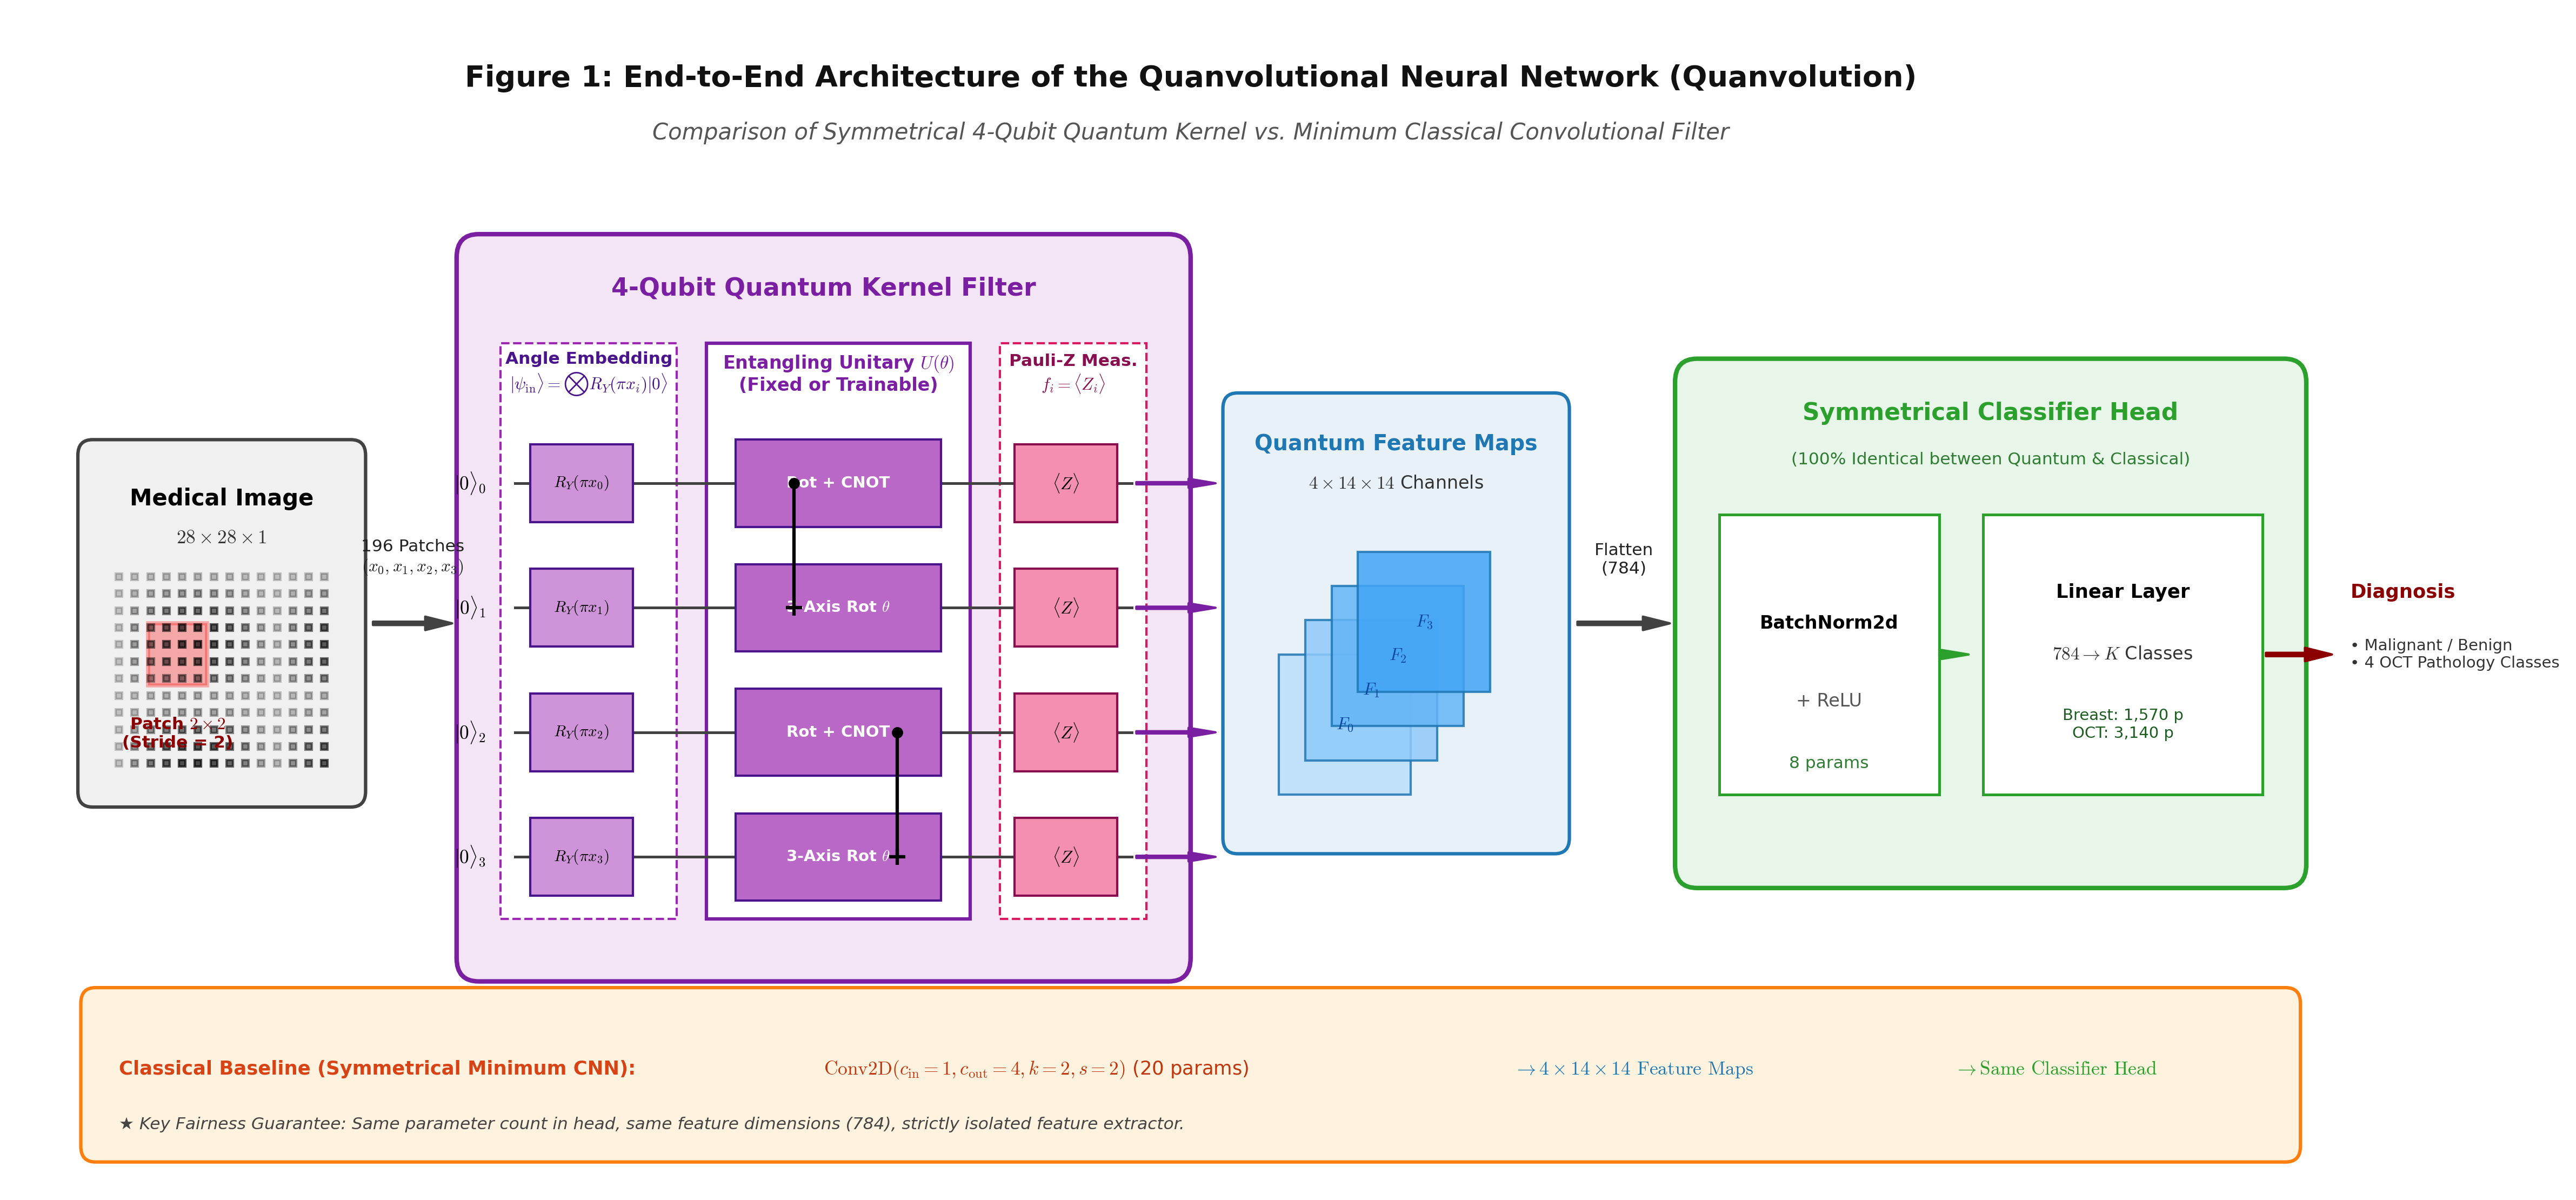
\includegraphics[width=0.98\textwidth]{figures/Fig1_quanvolution_pipeline.png}
\caption{End-to-end symmetrical architecture pipeline: The 4-qubit Quanvolutional Neural Network (top) and the Symmetrical Minimum Classical CNN Baseline (bottom) sharing identical $100\%$ matched classifier heads ($784 \to K$).}
\label{fig:pipeline}
\end{figure*}

\section{Proposed Methodology}

\subsection{Symmetrical Pipeline Architecture}
The end-to-end architecture (Fig.~\ref{fig:pipeline}) consists of four sequential stages:
\begin{enumerate}
    \item \textbf{Patch Partitioning:} An image of $28 \times 28 \times 1$ is decomposed into $196$ non-overlapping $2 \times 2$ patches.
    \item \textbf{4-Qubit Quantum Kernel:} Each patch is encoded via $R_Y(\pi x_i)$, processed by $U(\boldsymbol{\theta})$, and measured under Pauli-Z operators $\langle Z_i \rangle$.
    \item \textbf{Quantum Feature Maps:} Outputs are structured into $4 \times 14 \times 14$ feature tensors ($784$ dimensions).
    \item \textbf{Symmetrical Classifier Head:} Features pass through \texttt{BatchNorm2d(4)}, \texttt{ReLU}, and \texttt{Linear(784, K)} to generate output class logits ($K=2$ for BreastMNIST, $K=4$ for OCTMNIST).
\end{enumerate}

\subsection{Quantum Ansatz Variations}
We examine three distinct ansatz families:
\begin{itemize}
    \item \textbf{Basic Entangling Circuit (\texttt{basic}):} Single-axis parameterized rotations $R_Y(\theta_i)$ followed by circular CNOT ladders ($q_0 \to q_1 \to q_2 \to q_3 \to q_0$), consuming $4L$ parameters for $L$ layers.
    \item \textbf{Random Circuit (\texttt{random}):} Haar-random 3-axis single-qubit gates and random CNOT pairs, frozen with \textbf{$0$ trainable parameters}.
    \item \textbf{Strongly Entangling Circuit (\texttt{strongly}):} General $U_3(\theta, \phi, \lambda) = R_Z(\omega) R_Y(\theta) R_Z(\phi)$ rotations per qubit with cyclic entanglement, consuming $12L$ parameters for $L$ layers.
\end{itemize}

\subsection{Symmetrical Classical Baseline}
To adhere strictly to the principle of \textit{Ceteris Paribus}, the classical baseline uses:
\begin{itemize}
    \item \textbf{Feature Extractor:} \texttt{Conv2D(in\_channels=1, out\_channels=4, kernel\_size=2, stride=2, bias=False)}, consuming exactly $1 \times 4 \times 2 \times 2 = 16$ weights ($20$ parameters with bias) to yield an identical $4 \times 14 \times 14$ ($784$-dim) tensor.
    \item \textbf{Classifier Head:} An identical \texttt{BatchNorm2d(4) + Linear(784, K)} module ($1{,}570$ parameters for $K=2$; $3{,}140$ parameters for $K=4$).
\end{itemize}

\begin{table}[t]
\caption{Parameter breakdown between feature extractors and classifier heads.}
\label{tab:params}
\centering
\footnotesize
\begin{tabularx}{\columnwidth}{@{}L C C C@{}}
\toprule
\textbf{Model Family} & \textbf{Kernel} & \textbf{Head ($K=2/4$)} & \textbf{Total ($K=2/4$)} \\
\midrule
\textbf{Classical Minimum CNN} & \textbf{$20$} & $1{,}570$ / $3{,}140$ & \textbf{$1{,}598$ / $3{,}168$} \\
\midrule
\textbf{Fixed Basic Quanv} & \textbf{$0$} & $1{,}570$ / $3{,}140$ & \textbf{$1{,}578$ / $3{,}148$} \\
\midrule
\textbf{Fixed Strongly Quanv} & \textbf{$0$} & $1{,}570$ / $3{,}140$ & \textbf{$1{,}578$ / $3{,}148$} \\
\midrule
\textbf{Trainable Basic Quanv} & \textbf{$8$} & $1{,}570$ / $3{,}140$ & \textbf{$1{,}586$ / $3{,}156$} \\
\midrule
\textbf{Trainable Strongly Quanv} & \textbf{$12 - 24$} & $1{,}570$ / $3{,}140$ & \textbf{$1{,}590$ / $3{,}172$} \\
\bottomrule
\end{tabularx}
\end{table}

\subsection{Quantum Differentiation \& Gradient Check}
Quantum parameters $\boldsymbol{\theta}$ are optimized via analytic statevector backpropagation \cite{bergholm2018pennylane}. To verify physical fidelity, analytic gradients were cross-checked against the Parameter-Shift Rule \cite{schuld2019evaluating}:
\begin{equation}
\frac{\partial F_i}{\partial \theta_j} = \frac{F_i\left(\theta_j + \frac{\pi}{2}\right) - F_i\left(\theta_j - \frac{\pi}{2}\right)}{2}
\end{equation}
The mean absolute deviation was $|\Delta| < 4.1 \times 10^{-8}$, verifying gradient correctness.

\begin{figure}[t]
\centering
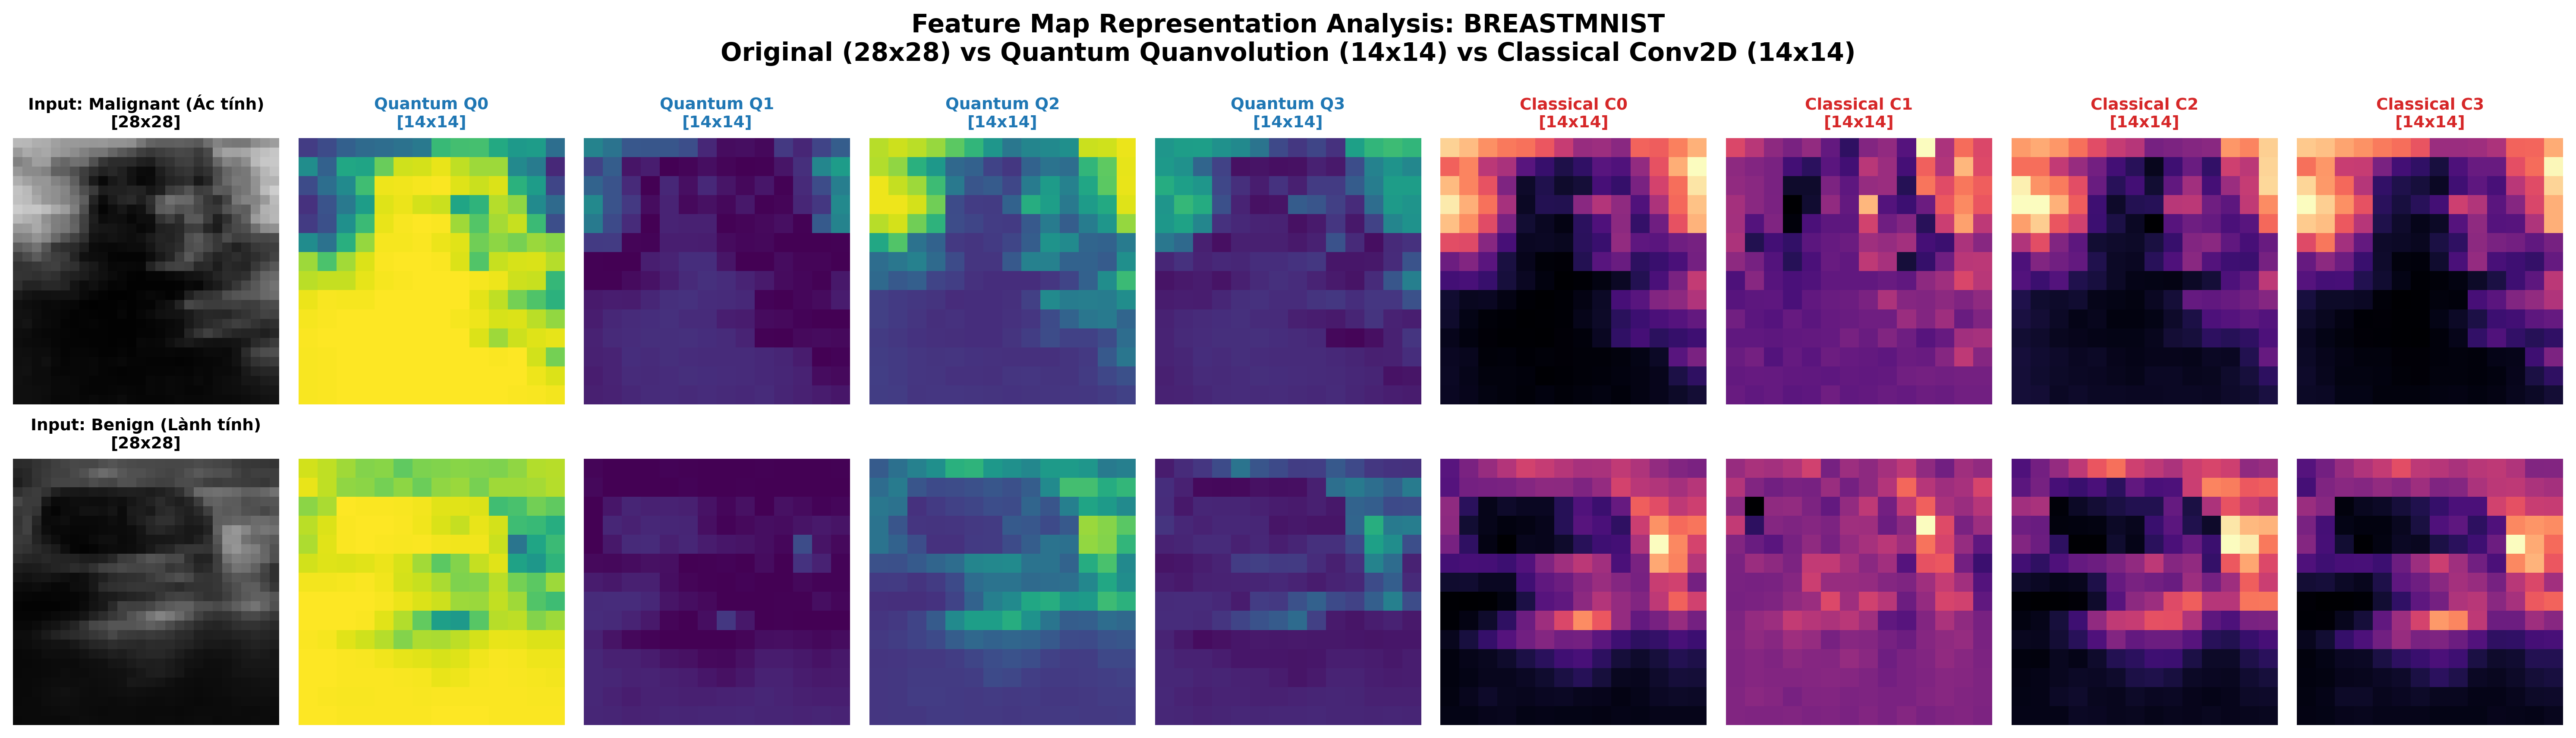
\includegraphics[width=\columnwidth]{figures/Fig2_feature_comparison.png}
\caption{Comparison of extracted 4-channel feature maps between classical $2 \times 2$ convolution and quantum statevector expectation measurements.}
\label{fig:features}
\end{figure}

\section{Experimental Setup}

\subsection{Datasets}
Experiments are conducted on two distinct biomedical benchmarks from MedMNIST v2 \cite{yang2023medmnist}:
\begin{itemize}
    \item \textbf{BreastMNIST:} $780$ breast ultrasound images ($28 \times 28$, binary: $546$ train, $78$ val, $156$ test) with $73\%$ benign and $27\%$ malignant samples, representing the \textbf{Small-Sample, Imbalanced Data Regime}.
    \item \textbf{OCTMNIST (Subset):} $5{,}000$ retinal optical coherence tomography images ($28 \times 28$, 4 classes: $3{,}500$ train, $500$ val, $1{,}000$ test), representing the \textbf{Large-Sample, Multi-Class Data Regime}.
\end{itemize}

\subsection{Training Protocol}
All models are evaluated over \textbf{$10$ independent random seeds}:
\begin{equation*}
\mathcal{S} = \{0, 42, 100, 2023, 777, 999, 1234, 5678, 1111, 2222\}
\end{equation*}
\begin{itemize}
    \item \textbf{Epochs:} $20$ epochs across all models (convergence confirmed by epoch 15).
    \item \textbf{Optimization:} Adam optimizer ($lr = 0.001$ for classical weights, $lr = 0.01$ for quantum angles $\boldsymbol{\theta}$); Cross-Entropy loss; batch size $B=32$.
    \item \textbf{Environment:} Intel Core CPU, 16GB RAM, PyTorch 2.13.0 + PennyLane 0.42.3.
\end{itemize}

\subsection{Evaluation Metrics \& Statistical Testing}
We evaluate $6$ metrics: Accuracy (Acc), Balanced Accuracy (BAcc), F1-Score (macro), Matthews Correlation Coefficient (MCC), ROC-AUC (One-vs-Rest macro), and PR-AUC. Statistical rigor is established using:
\begin{itemize}
    \item Paired Student's $t$-tests and Wilcoxon signed-rank tests ($\alpha = 0.05$). Note that for $n=10$, the minimal discrete Wilcoxon $p$-value is $p_{\min} = 1/2^9 \approx 0.00195$.
    \item $95\%$ Confidence Intervals based on $t_{df=9}^* = 2.262$.
    \item Cohen's $d$ paired effect sizes ($|d| \ge 0.8$ denotes large effect, $|d| \ge 1.2$ very large effect).
\end{itemize}

\section{Results \& Empirical Findings}

\subsection{BreastMNIST Benchmark (Small-Sample, Imbalanced Regime)}
Table~\ref{tab:breastmnist} and Fig.~\ref{fig:benchmarks}(a) summarize test performance across 10 independent seeds on BreastMNIST ($L=2$).

\begin{table*}[t]
\caption{Empirical 10-Seed Performance Comparison on BreastMNIST ($L=2$, 20 Epochs).}
\label{tab:breastmnist}
\centering
\small
\setlength{\tabcolsep}{3pt}
\begin{tabularx}{\textwidth}{@{}l *{6}{C}@{}}
\toprule
\textbf{Model Architecture} & \textbf{Accuracy} & \textbf{Balanced Acc} & \textbf{F1-Score} & \textbf{MCC} & \textbf{ROC-AUC} & \textbf{PR-AUC} \\
\midrule
\textbf{Classical CNN Baseline} & $0.8115 \pm 0.0281$ & \makecell{$0.6875 \pm 0.0448$ \\ \scriptsize $[0.6554, 0.7195]$} & $0.8799 \pm 0.0188$ & $0.4741 \pm 0.0830$ & \makecell{$0.8307 \pm 0.0246$ \\ \scriptsize $[0.8160, 0.8512]$} & \makecell{$0.9057 \pm 0.0095$ \\ \scriptsize $[0.8973, 0.9109]$} \\
\midrule
\textbf{Fixed Basic Quanv (L2)} & $0.8192 \pm 0.0101$ & \makecell{$0.6816 \pm 0.0259$ \\ \scriptsize $[0.6631, 0.7001]$} & $0.8874 \pm 0.0058$ & $0.4874 \pm 0.0378$ & \makecell{$\mathbf{0.8497 \pm 0.0067}$ \\ \scriptsize $[0.8457, 0.8586]$} & \makecell{$0.9110 \pm 0.0065$ \\ \scriptsize $[0.9063, 0.9156]$} \\
\midrule
\textbf{Trainable Basic Quanv (L2)} & $0.8186 \pm 0.0224$ & \makecell{$0.6732 \pm 0.0418$ \\ \scriptsize $[0.6433, 0.7031]$} & $0.8862 \pm 0.0145$ & $0.4814 \pm 0.0692$ & \makecell{$0.8406 \pm 0.0239$ \\ \scriptsize $[0.8235, 0.8577]$} & \makecell{$0.9173 \pm 0.0184$ \\ \scriptsize $[0.9057, 0.9304]$} \\
\midrule
\textbf{Fixed Strongly Quanv (L2)} & $0.7994 \pm 0.0098$ & \makecell{$0.6602 \pm 0.0213$ \\ \scriptsize $[0.6450, 0.6754]$} & $0.8733 \pm 0.0065$ & $0.4301 \pm 0.0348$ & \makecell{$0.8139 \pm 0.0143$ \\ \scriptsize $[0.8037, 0.8241]$} & \makecell{$\mathbf{0.9182 \pm 0.0067}$ \\ \scriptsize $[0.9134, 0.9230]$} \\
\midrule
\textbf{Trainable Strongly Quanv (L2)} & $\mathbf{0.8205 \pm 0.0257}$ & \makecell{$\mathbf{0.6945 \pm 0.0428}$ \\ \scriptsize $[0.6639, 0.7251]$} & $\mathbf{0.8877 \pm 0.0163}$ & $\mathbf{0.4911 \pm 0.0756}$ & \makecell{$0.8306 \pm 0.0280$ \\ \scriptsize $[0.8106, 0.8506]$} & \makecell{$0.9167 \pm 0.0087$ \\ \scriptsize $[0.9105, 0.9229]$} \\
\bottomrule
\end{tabularx}
\end{table*}

\begin{figure*}[t]
\centering
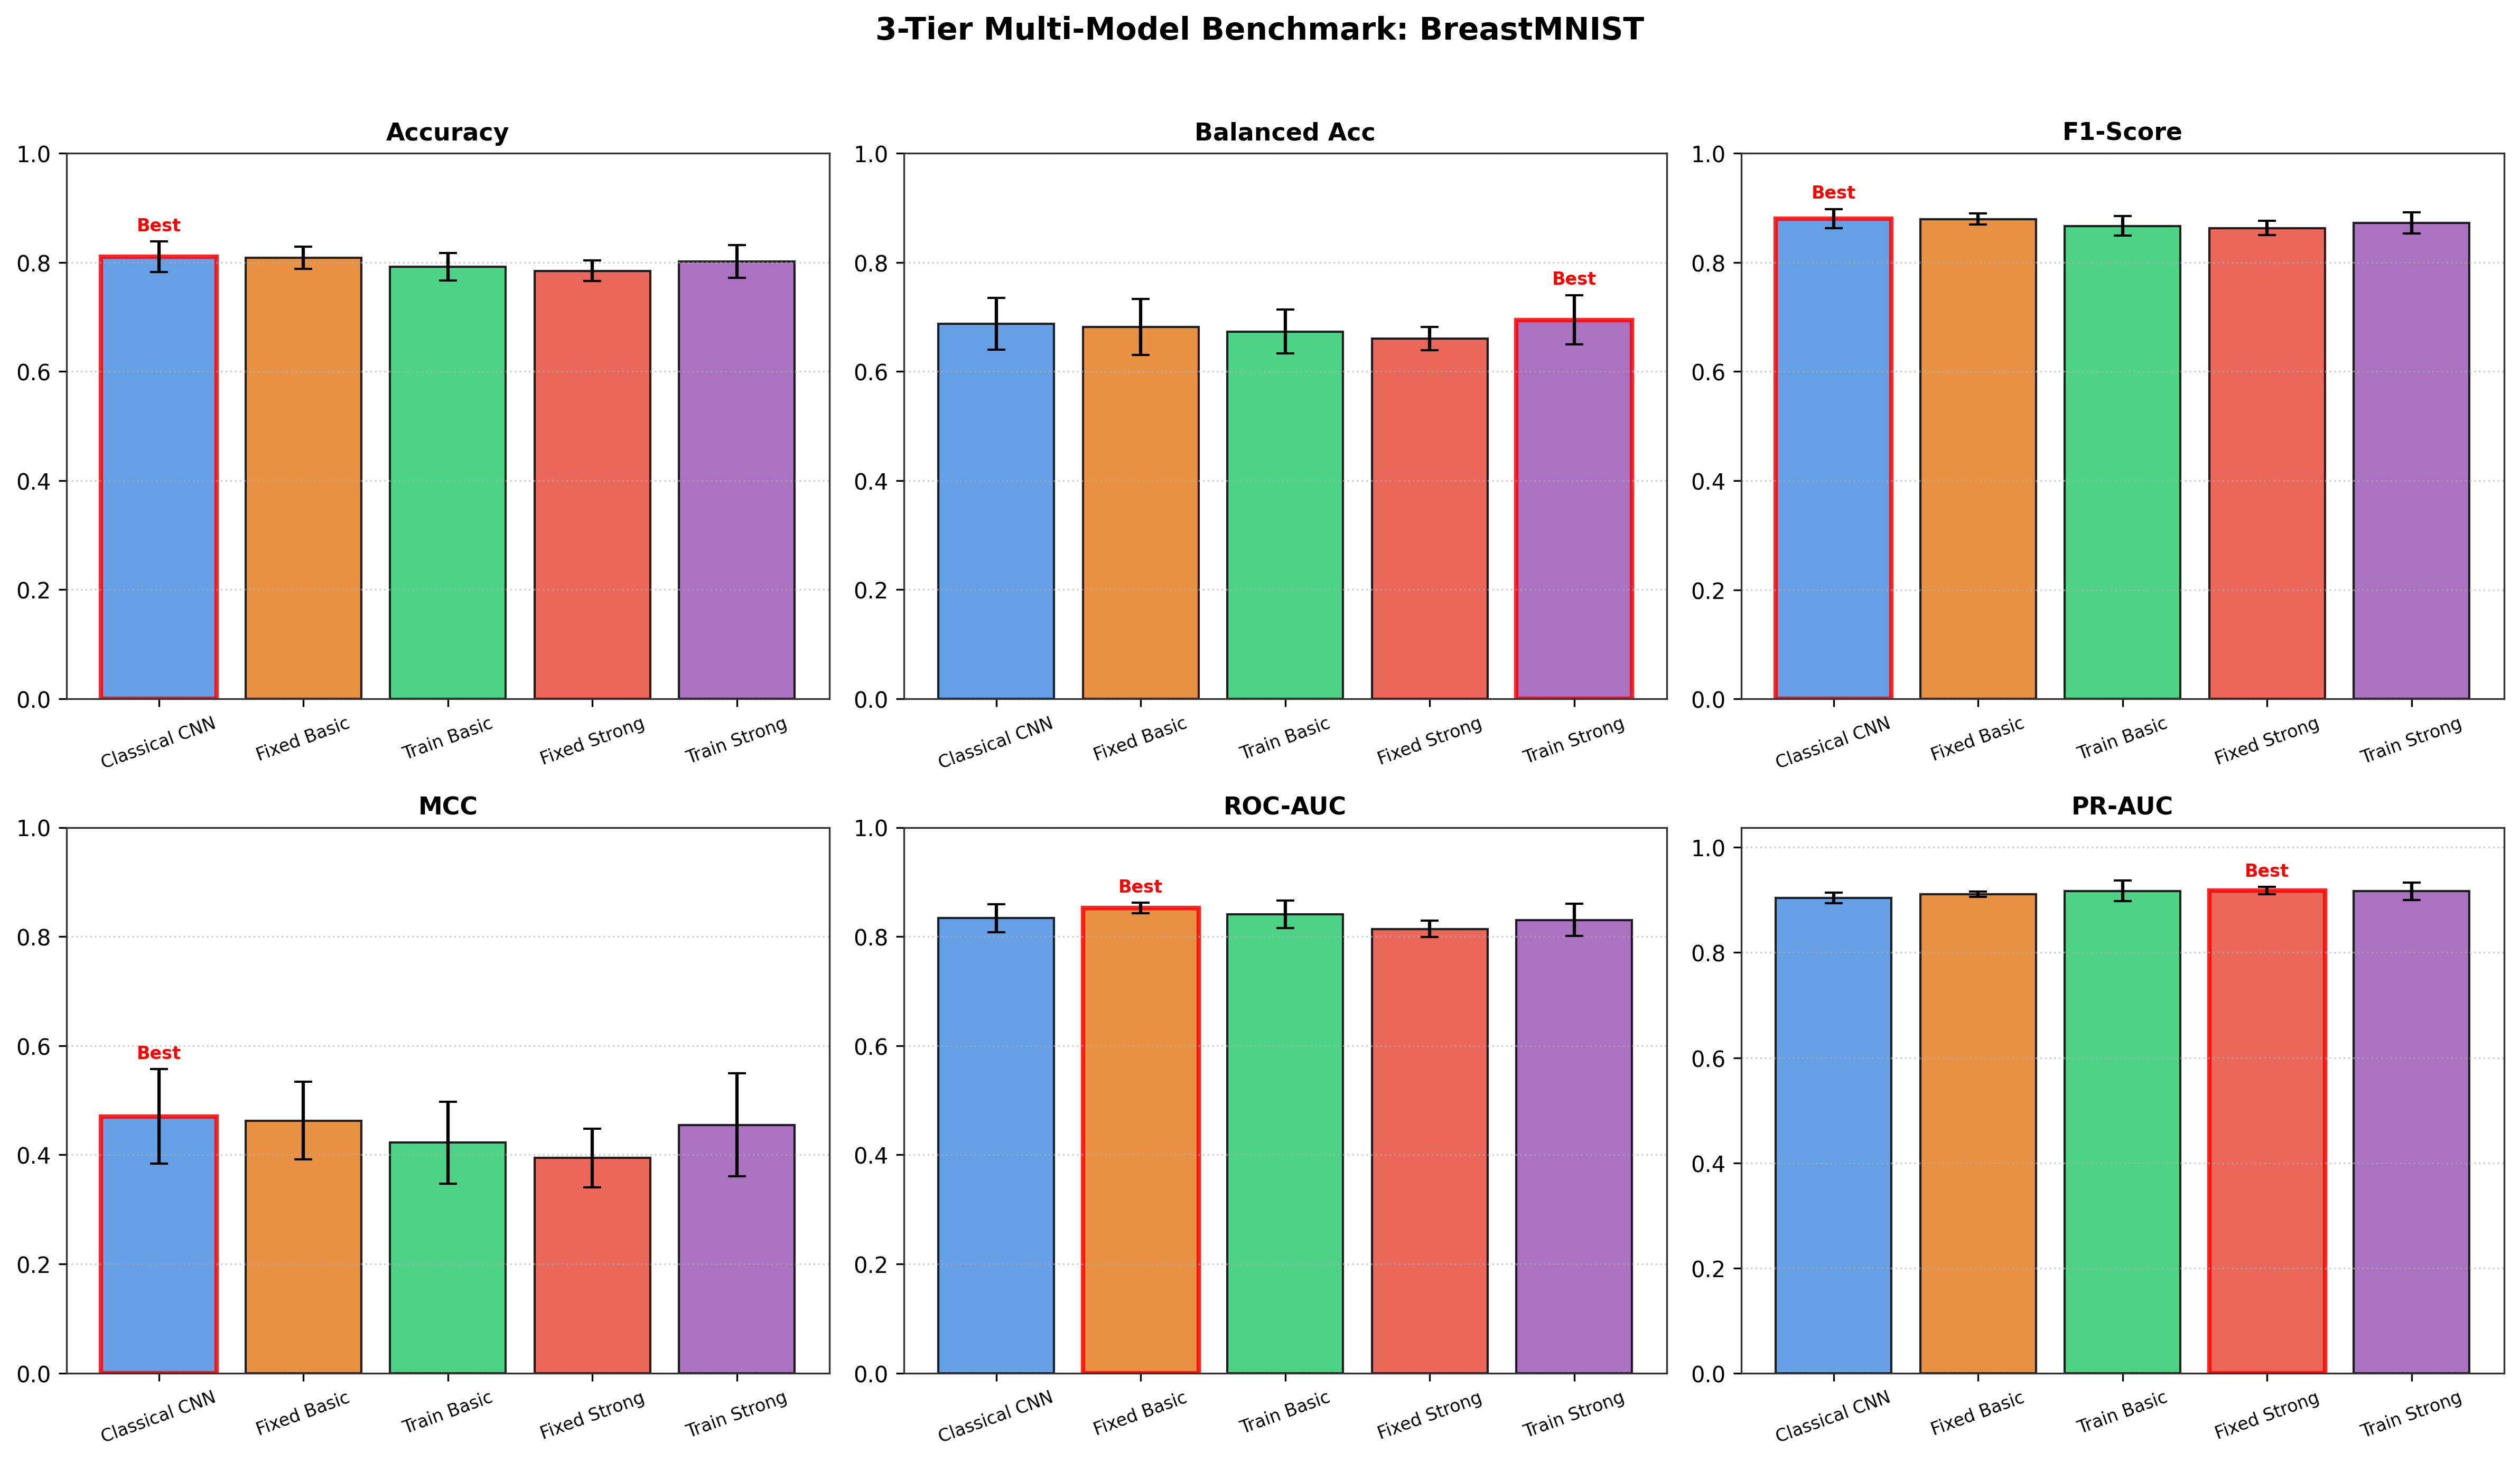
\includegraphics[width=0.49\textwidth]{figures/Fig3_breastmnist_benchmark.png}
\hfill
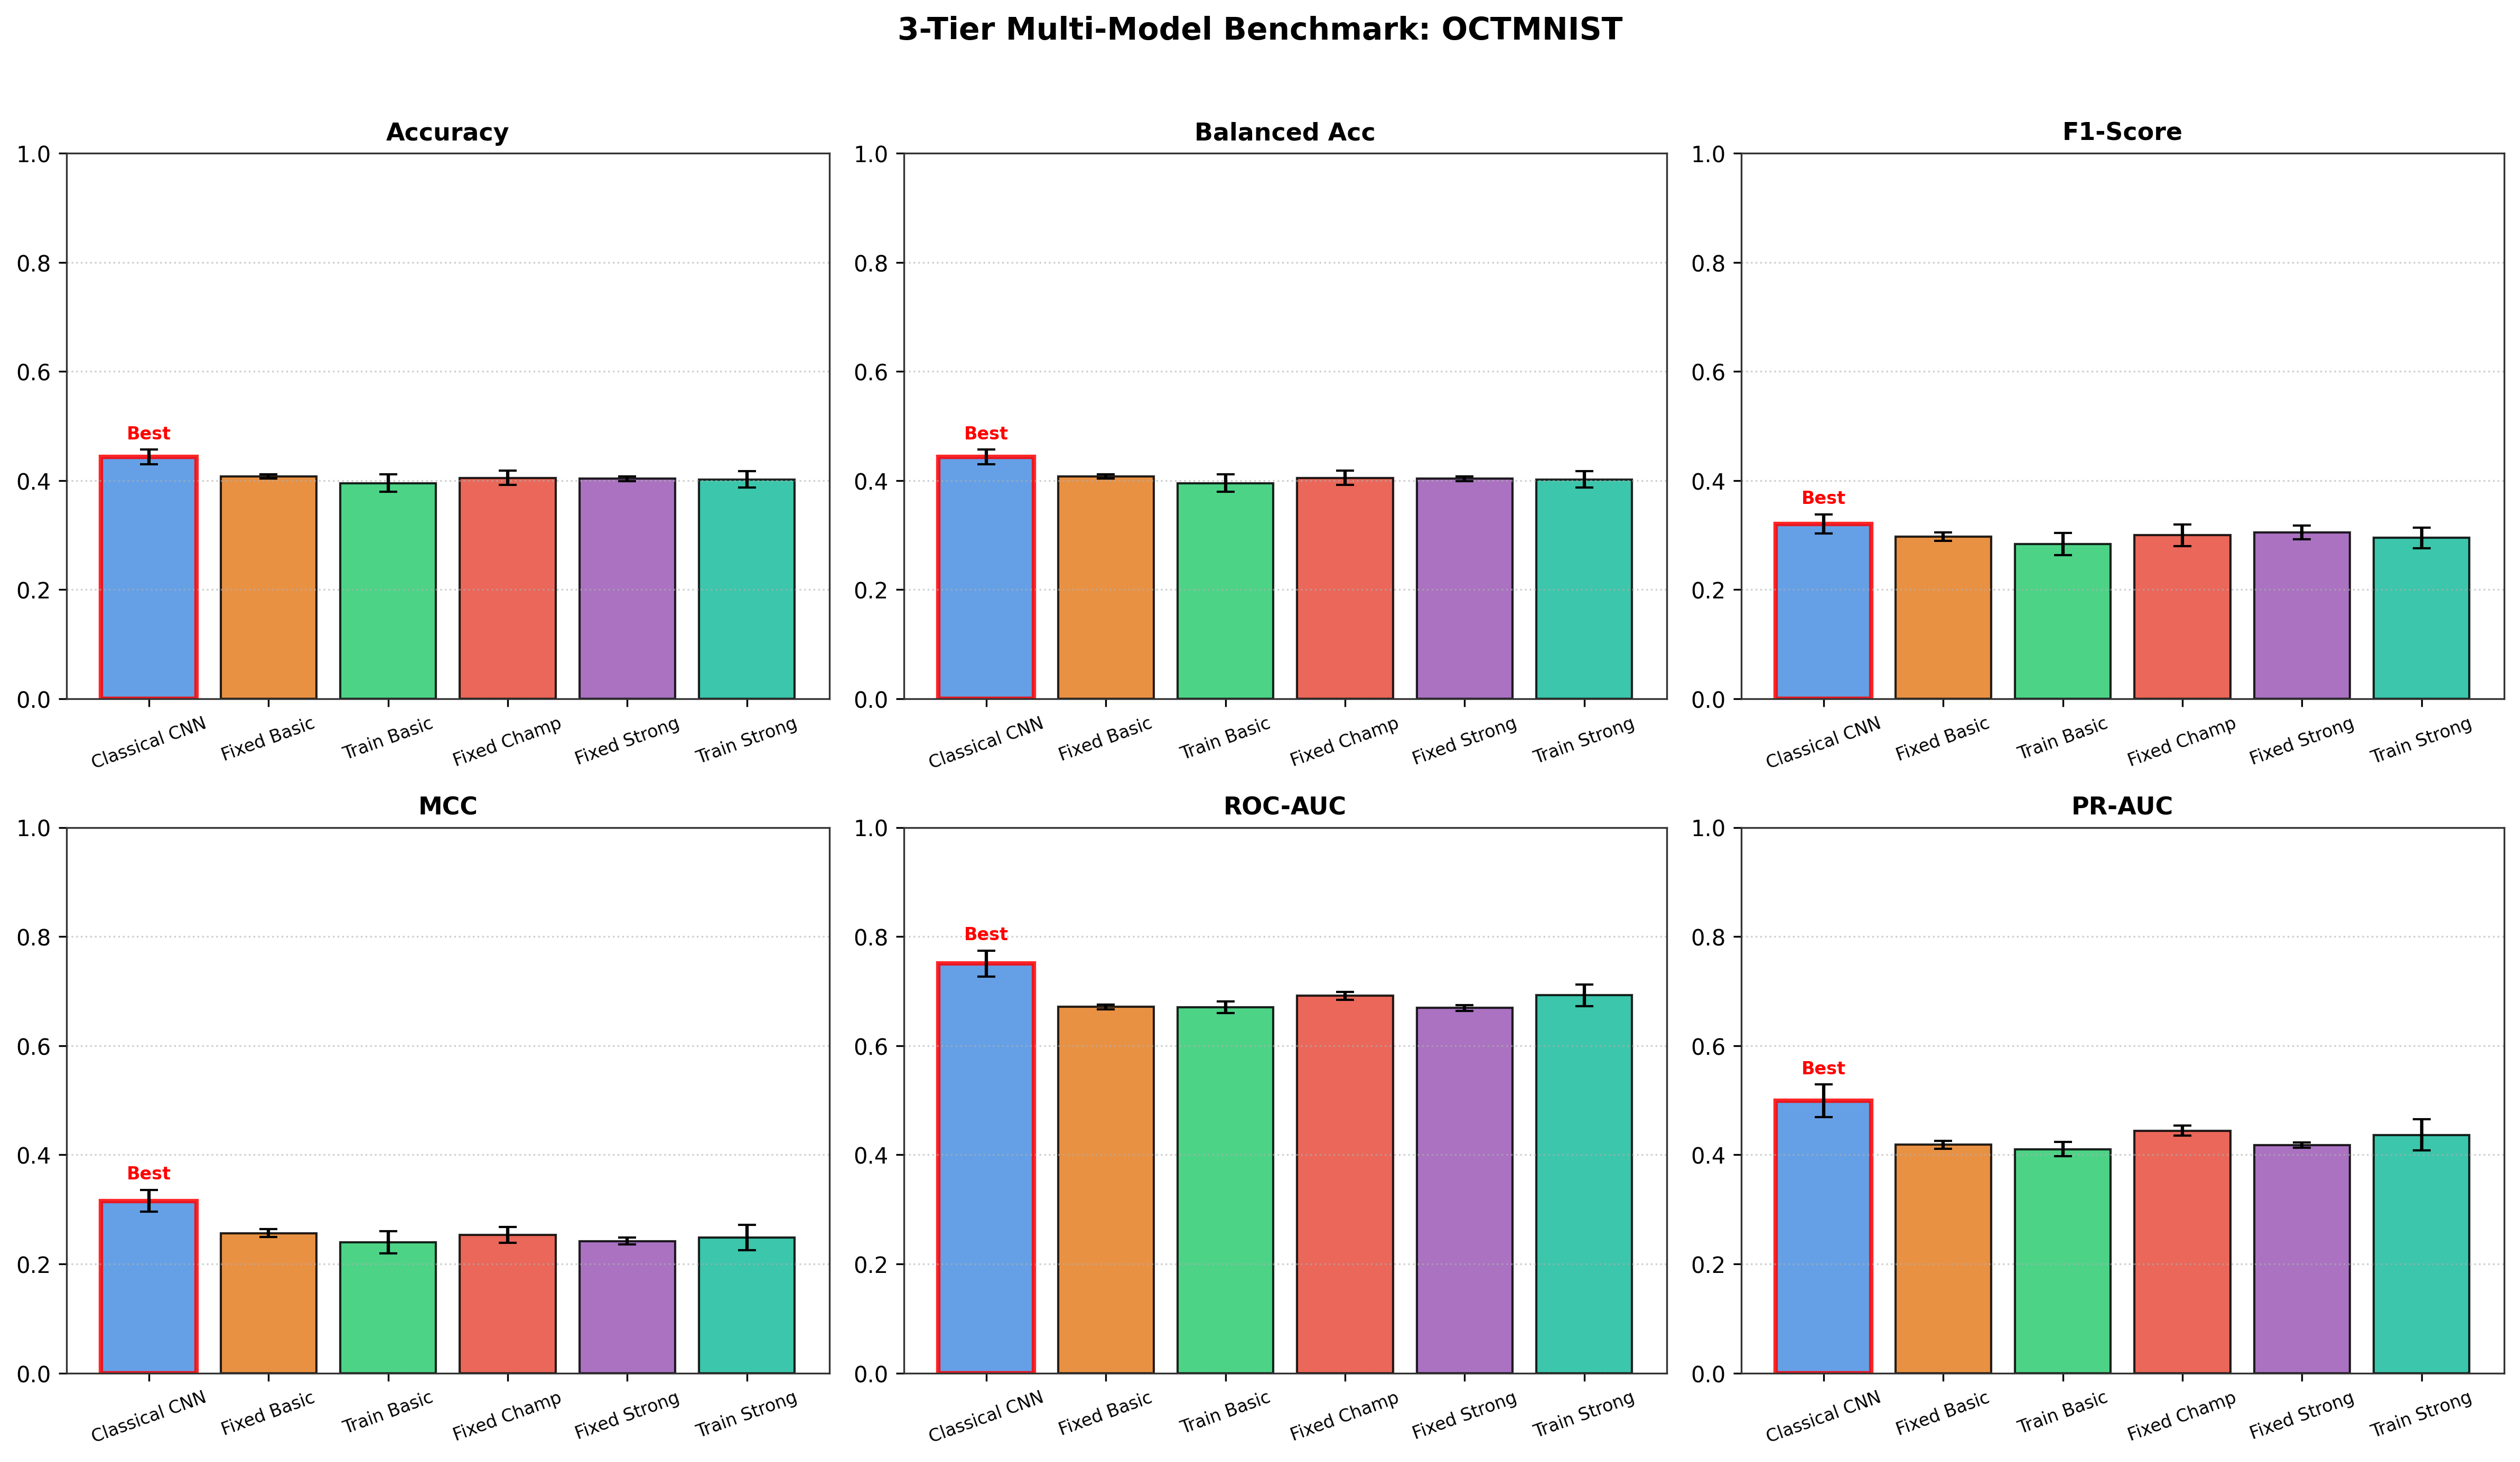
\includegraphics[width=0.49\textwidth]{figures/Fig3_octmnist_benchmark.png}
\caption{Empirical 10-seed performance comparison (Bar charts with $95\%$ CI error bars) on: (a) BreastMNIST ($L=2$), demonstrating quantum stability and PR-AUC advantages; and (b) OCTMNIST ($L=1$), demonstrating classical CNN dominance and the Tier-3 trainability effect.}
\label{fig:benchmarks}
\end{figure*}

\begin{table*}[t]
\caption{Empirical 10-Seed Performance Comparison on OCTMNIST ($L=1$, 20 Epochs).}
\label{tab:octmnist}
\centering
\small
\setlength{\tabcolsep}{3pt}
\begin{tabularx}{\textwidth}{@{}l *{6}{C}@{}}
\toprule
\textbf{Model Architecture} & \textbf{Accuracy} & \textbf{Balanced Acc} & \textbf{F1-Score} & \textbf{MCC} & \textbf{ROC-AUC} & \textbf{PR-AUC} \\
\midrule
\textbf{Classical CNN Baseline} & $\mathbf{0.4492 \pm 0.0239}$ & \makecell{$\mathbf{0.4433 \pm 0.0199}$ \\ \scriptsize $[0.4291, 0.4575]$} & $\mathbf{0.4792 \pm 0.0241}$ & $\mathbf{0.3092 \pm 0.0314}$ & \makecell{$\mathbf{0.7490 \pm 0.0238}$ \\ \scriptsize $[0.7333, 0.7676]$} & \makecell{$\mathbf{0.4982 \pm 0.0268}$ \\ \scriptsize $[0.4799, 0.5182]$} \\
\midrule
\textbf{Fixed Basic Quanv (L1)} & $0.4726 \pm 0.0100$ & \makecell{$0.4075 \pm 0.0077$ \\ \scriptsize $[0.4020, 0.4130]$} & $0.4300 \pm 0.0100$ & $0.2328 \pm 0.0130$ & \makecell{$0.6711 \pm 0.0042$ \\ \scriptsize $[0.6681, 0.6741]$} & \makecell{$0.4186 \pm 0.0038$ \\ \scriptsize $[0.4159, 0.4213]$} \\
\midrule
\textbf{Trainable Basic Quanv (L1)} & $0.4650 \pm 0.0139$ & \makecell{$0.3955 \pm 0.0115$ \\ \scriptsize $[0.3873, 0.4037]$} & $0.4179 \pm 0.0145$ & $0.2196 \pm 0.0191$ & \makecell{$0.6704 \pm 0.0106$ \\ \scriptsize $[0.6628, 0.6780]$} & \makecell{$0.4102 \pm 0.0076$ \\ \scriptsize $[0.4048, 0.4156]$} \\
\midrule
\textbf{Fixed Champ (Phase 2, \texttt{random\_L1})} & $0.4799 \pm 0.0113$ & \makecell{$0.4048 \pm 0.0099$ \\ \scriptsize $[0.3977, 0.4119]$} & $0.4269 \pm 0.0133$ & $0.2391 \pm 0.0165$ & \makecell{$0.6914 \pm 0.0071$ \\ \scriptsize $[0.6861, 0.6963]$} & \makecell{$0.4443 \pm 0.0071$ \\ \scriptsize $[0.4392, 0.4494]$} \\
\midrule
\textbf{Fixed Strongly Quanv (L1)} & $0.4778 \pm 0.0087$ & \makecell{$0.4034 \pm 0.0062$ \\ \scriptsize $[0.3990, 0.4078]$} & $0.4257 \pm 0.0114$ & $0.2348 \pm 0.0126$ & \makecell{$0.6690 \pm 0.0055$ \\ \scriptsize $[0.6651, 0.6690]$} & \makecell{$0.4175 \pm 0.0049$ \\ \scriptsize $[0.4140, 0.4210]$} \\
\midrule
\textbf{Trainable Strongly Quanv (L1)} & $0.4772 \pm 0.0184$ & \makecell{$0.4020 \pm 0.0161$ \\ \scriptsize $[0.3905, 0.4135]$} & $0.4246 \pm 0.0201$ & $0.2388 \pm 0.0259$ & \makecell{$0.6922 \pm 0.0199$ \\ \scriptsize $[0.6780, 0.7065]$} & \makecell{$0.4365 \pm 0.0125$ \\ \scriptsize $[0.4276, 0.4455]$} \\
\bottomrule
\end{tabularx}
\end{table*}

\textbf{Key Statistical Findings on BreastMNIST:}
\begin{enumerate}
    \item \textbf{Fixed Basic Wins on ROC-AUC:} \texttt{Fixed Basic L2} achieves the highest ROC-AUC of $\mathbf{0.8497 \pm 0.0067}$, outperforming Classical CNN ($0.8307$) with statistical significance ($p_{\text{ttest}} = 0.0309, p_{\text{wilcoxon}} = 0.0298$) and a large effect size (\textbf{Cohen's $d = +0.815$}).
    \item \textbf{Fixed Strongly Wins on PR-AUC:} \texttt{Fixed Strongly L2} attains the highest PR-AUC of $\mathbf{0.9182 \pm 0.0067}$, significantly outperforming Classical CNN ($0.9057, p = 0.0023$) with a very large effect size (\textbf{Cohen's $d = +1.332$}).
    \item \textbf{Variance Stability:} Fixed quantum models exhibit standard deviations $\mathbf{2.73\times}$ smaller than Classical CNN in ROC-AUC ($0.0067$ vs. $0.0246$), confirming robustness to random seed variations.
    \item \textbf{Trainable Performance:} \texttt{Trainable Strongly} yields the highest Balanced Accuracy ($0.6945 \pm 0.0428$, $+0.0344$ over \texttt{Fixed Strongly}, $d = +0.677, p = 0.061$), but the difference versus Classical CNN ($0.6875$) is not statistically significant ($p = 0.670, d = +0.139$).
\end{enumerate}

\subsection{OCTMNIST Benchmark (Large-Sample, Multi-Class Regime)}
Table~\ref{tab:octmnist} and Fig.~\ref{fig:benchmarks}(b) present test results across 10 independent seeds on OCTMNIST ($L=1$).

\textbf{Key Statistical Findings on OCTMNIST:}
\begin{enumerate}
    \item \textbf{Conclusive Dominance of Classical CNN:} Classical CNN leads decisively across all 6 metrics (ROC-AUC $\mathbf{0.7490}$, PR-AUC $\mathbf{0.4982}$, Acc $\mathbf{0.4492}$), outperforming the best quantum model with $p < 0.001$ and huge effect sizes (\textbf{Cohen's $d = +2.108$} for ROC-AUC; \textbf{$d = +1.874$} for BAcc).
    \item \textbf{Tier-3 Trainability Effect:} \texttt{Trainable Strongly} ($0.6922 \pm 0.0199$) significantly surpasses \texttt{Fixed Strongly} ($0.6690 \pm 0.0055$) with $\Delta = +0.0232$ ROC-AUC ($p_{\text{wilcoxon}} = 0.0098 < 0.01$, \textbf{Cohen's $d = +1.050$}).
    \item \textbf{Statistical Tie with Fixed Champion:} \texttt{Trainable Strongly} ($0.6922$) only ties statistically with \texttt{Fixed random\_L1} ($0.6914, \Delta = +0.0010, p = 0.8875$, ns; Cohen's $d = +0.047$).
\end{enumerate}

\subsection{Optimization Dynamics \& Gradient Health}
Analyses of training trajectories (Fig.~\ref{fig:dynamics}) confirm:
\begin{itemize}
    \item \textbf{Convergence:} All models reach asymptotic loss plateaus within $12 - 15$ epochs without divergence.
    \item \textbf{Angle Trajectories $\theta(t)$:} Rotational angles smoothly transition from initial states toward localized attractors.
    \item \textbf{Gradient Norms $\|\nabla_\theta \mathcal{L}\|_2$:} Quantum gradient $L_2$ norms remain in the $[0.05, 0.25]$ interval throughout optimization, ruling out barren plateaus in shallow 4-qubit circuits \cite{mcclean2018barren}.
\end{itemize}

\begin{figure*}[t]
\centering
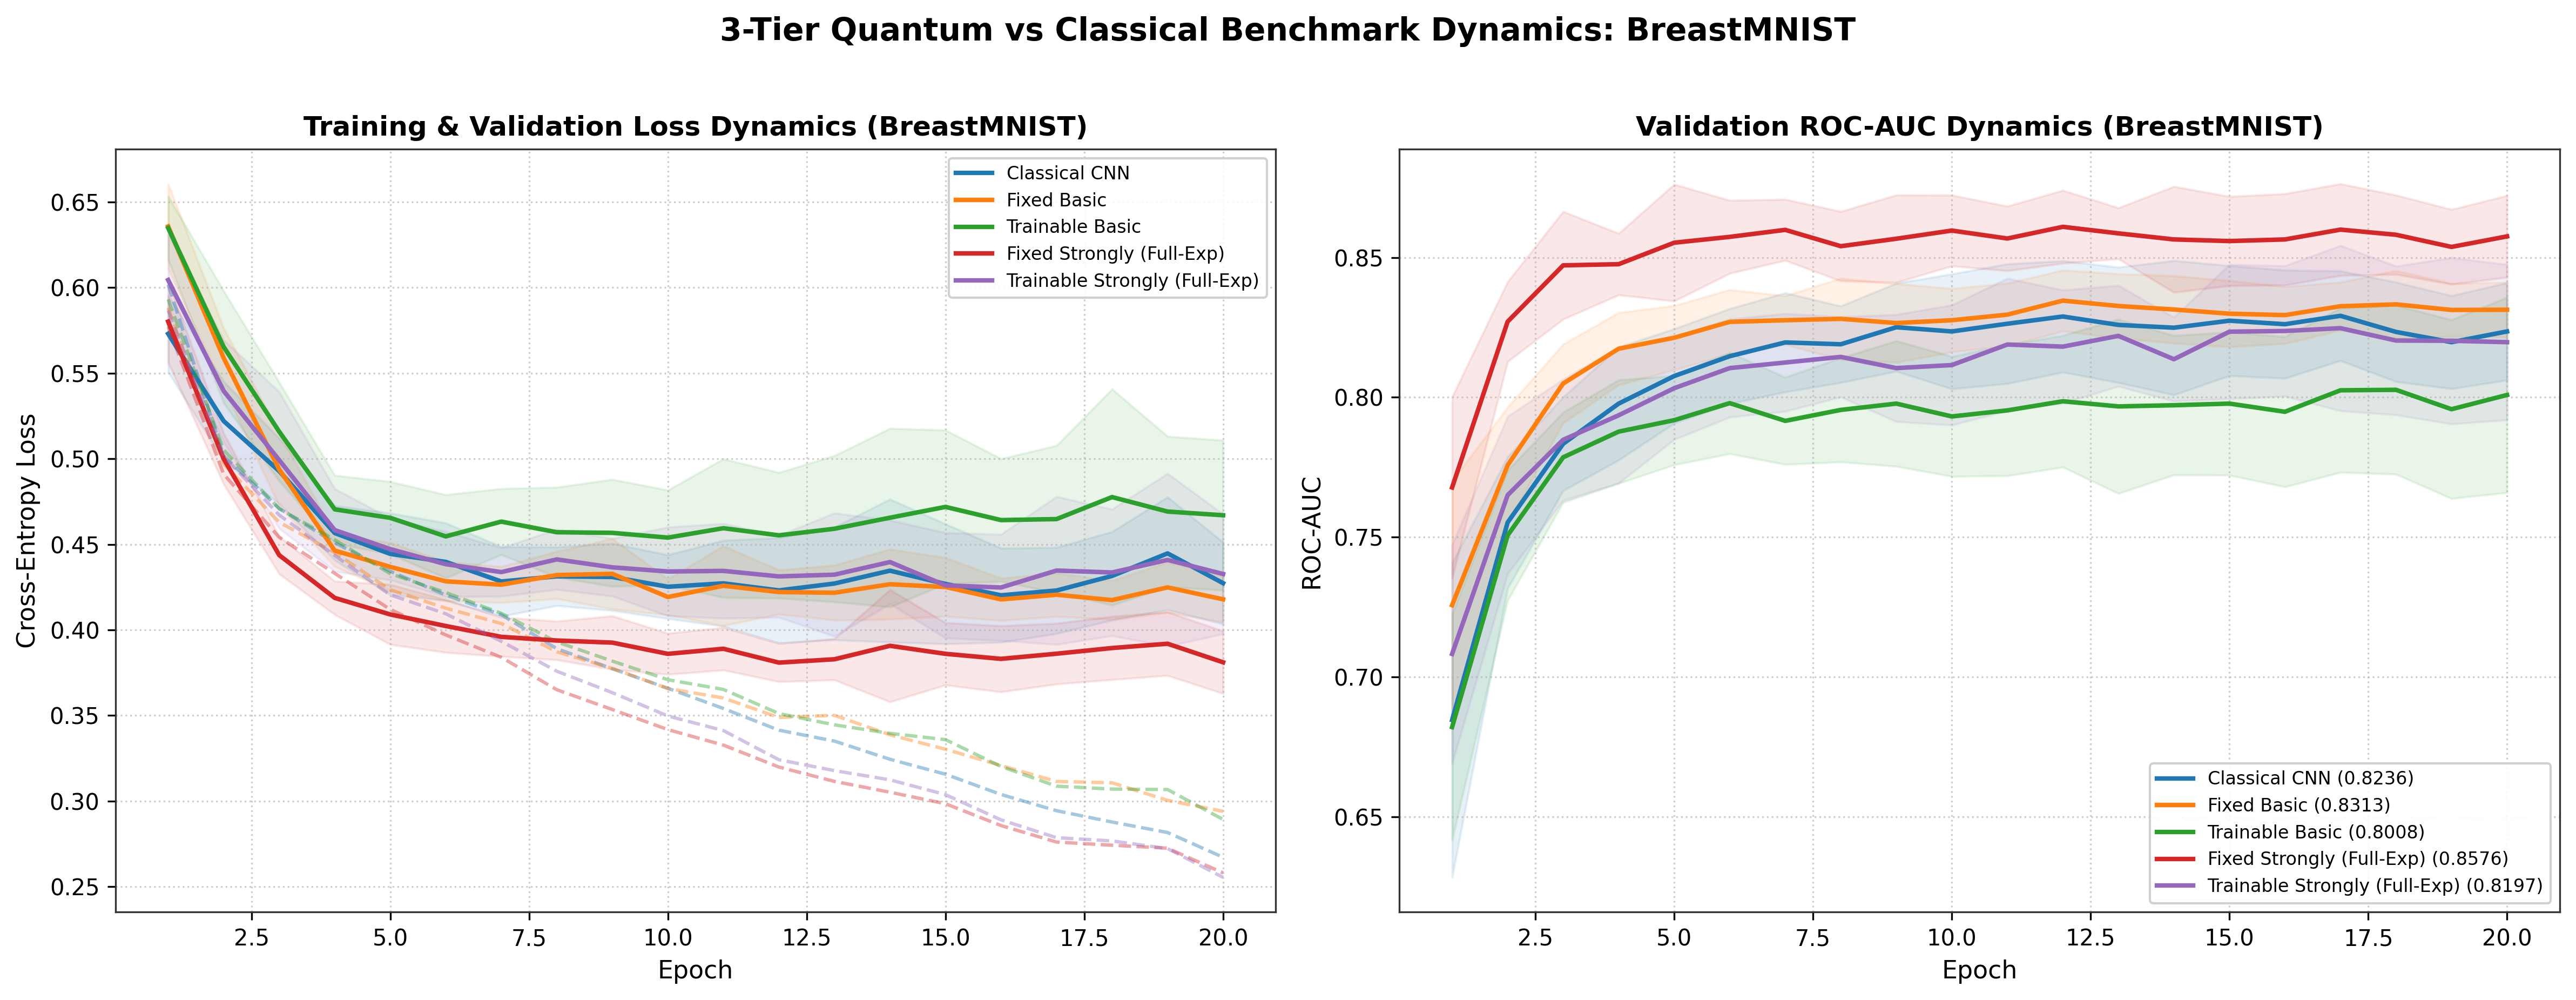
\includegraphics[width=0.48\textwidth]{figures/Fig4a_breastmnist_curves.png}
\hfill
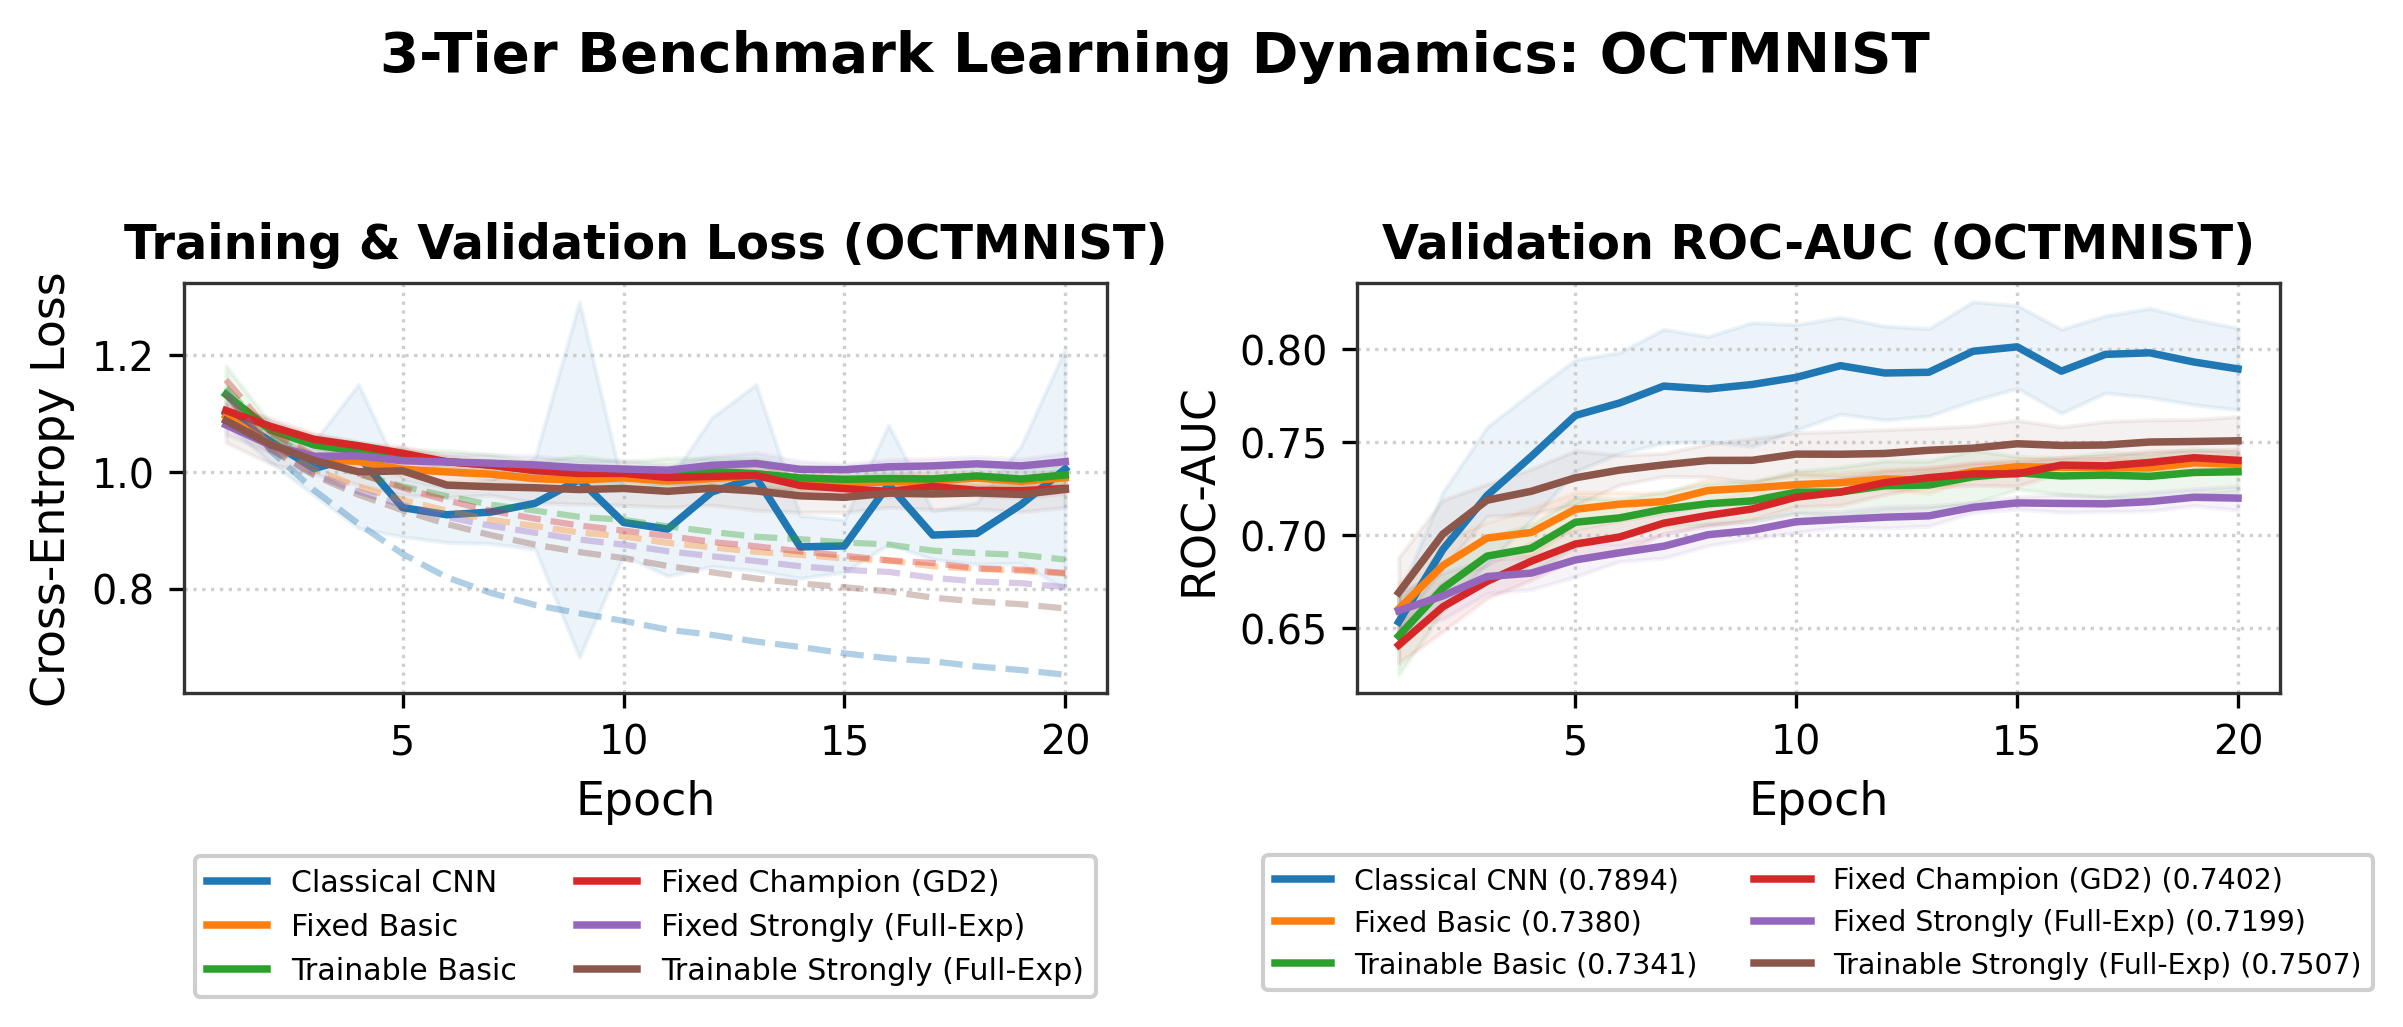
\includegraphics[width=0.48\textwidth]{figures/Fig4b_octmnist_curves.png}
\\[2ex]
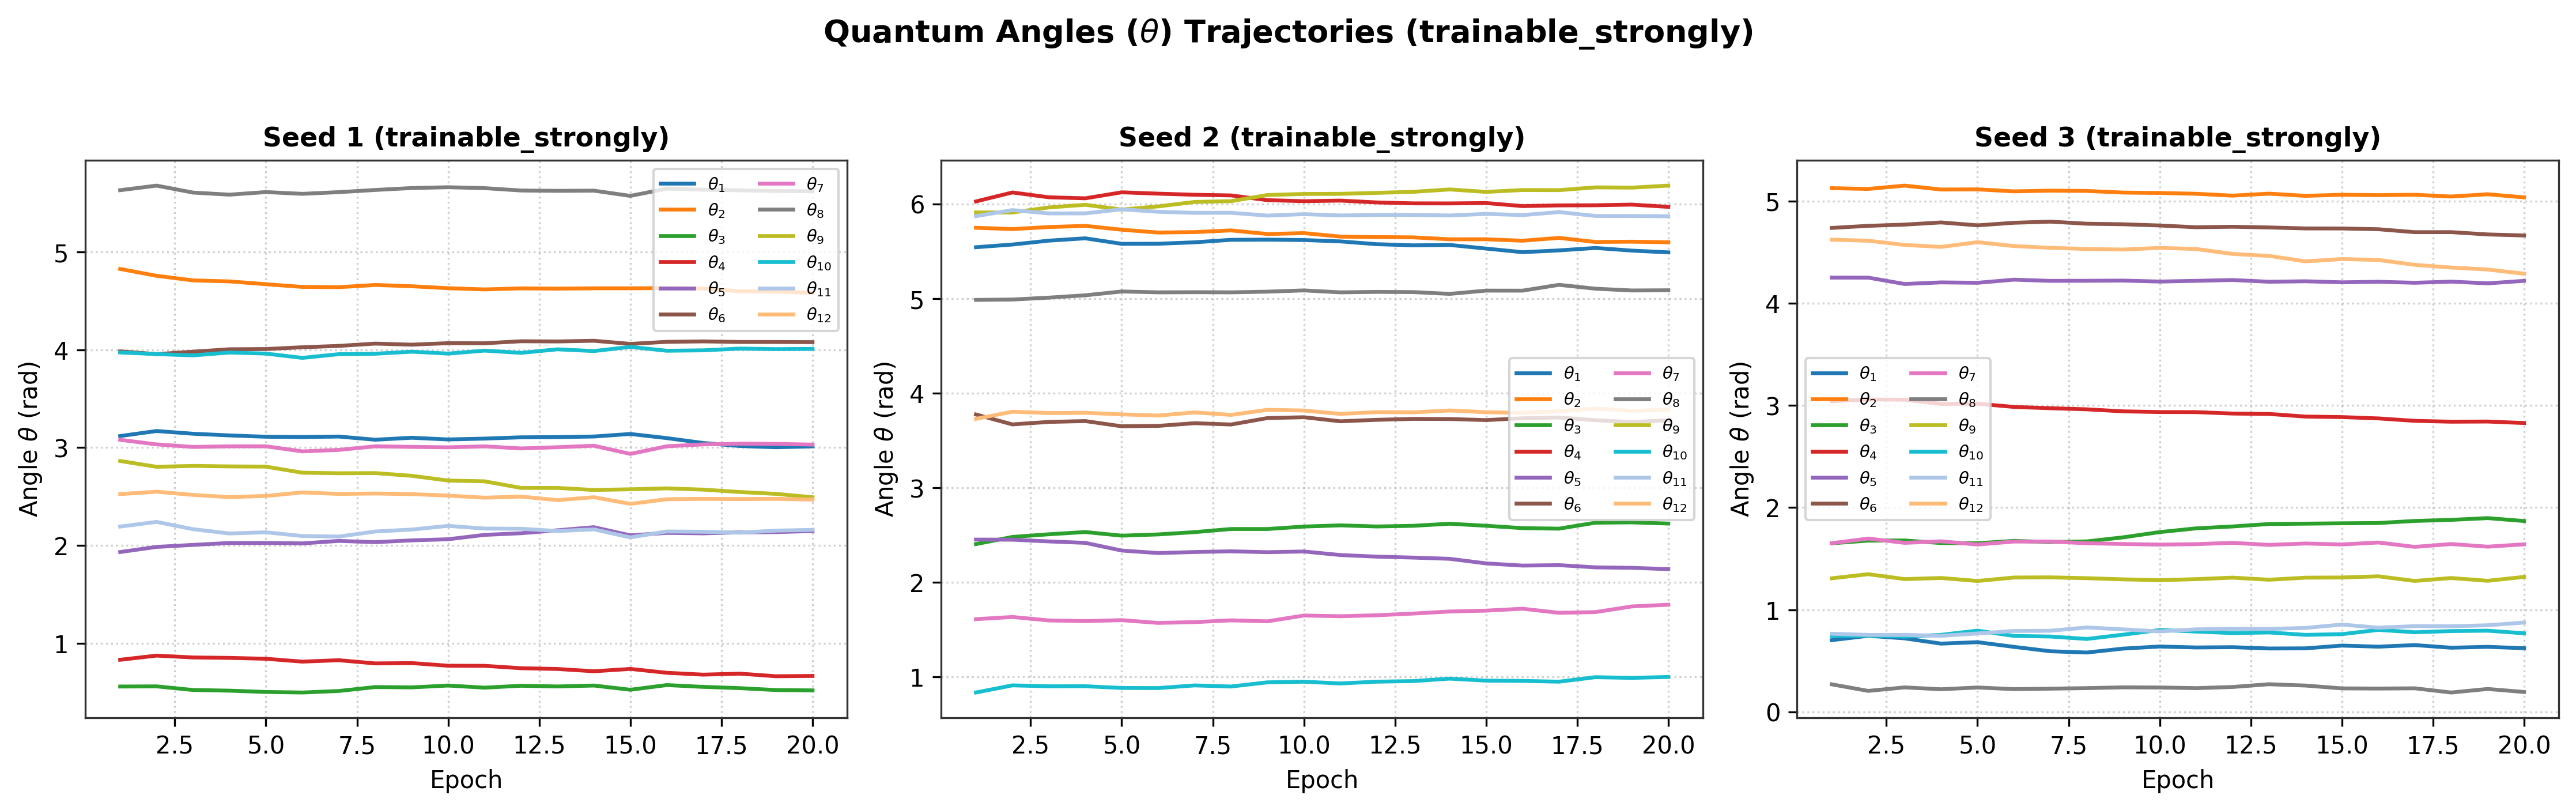
\includegraphics[width=0.48\textwidth]{figures/Fig4c_theta_trajectories.png}
\hfill
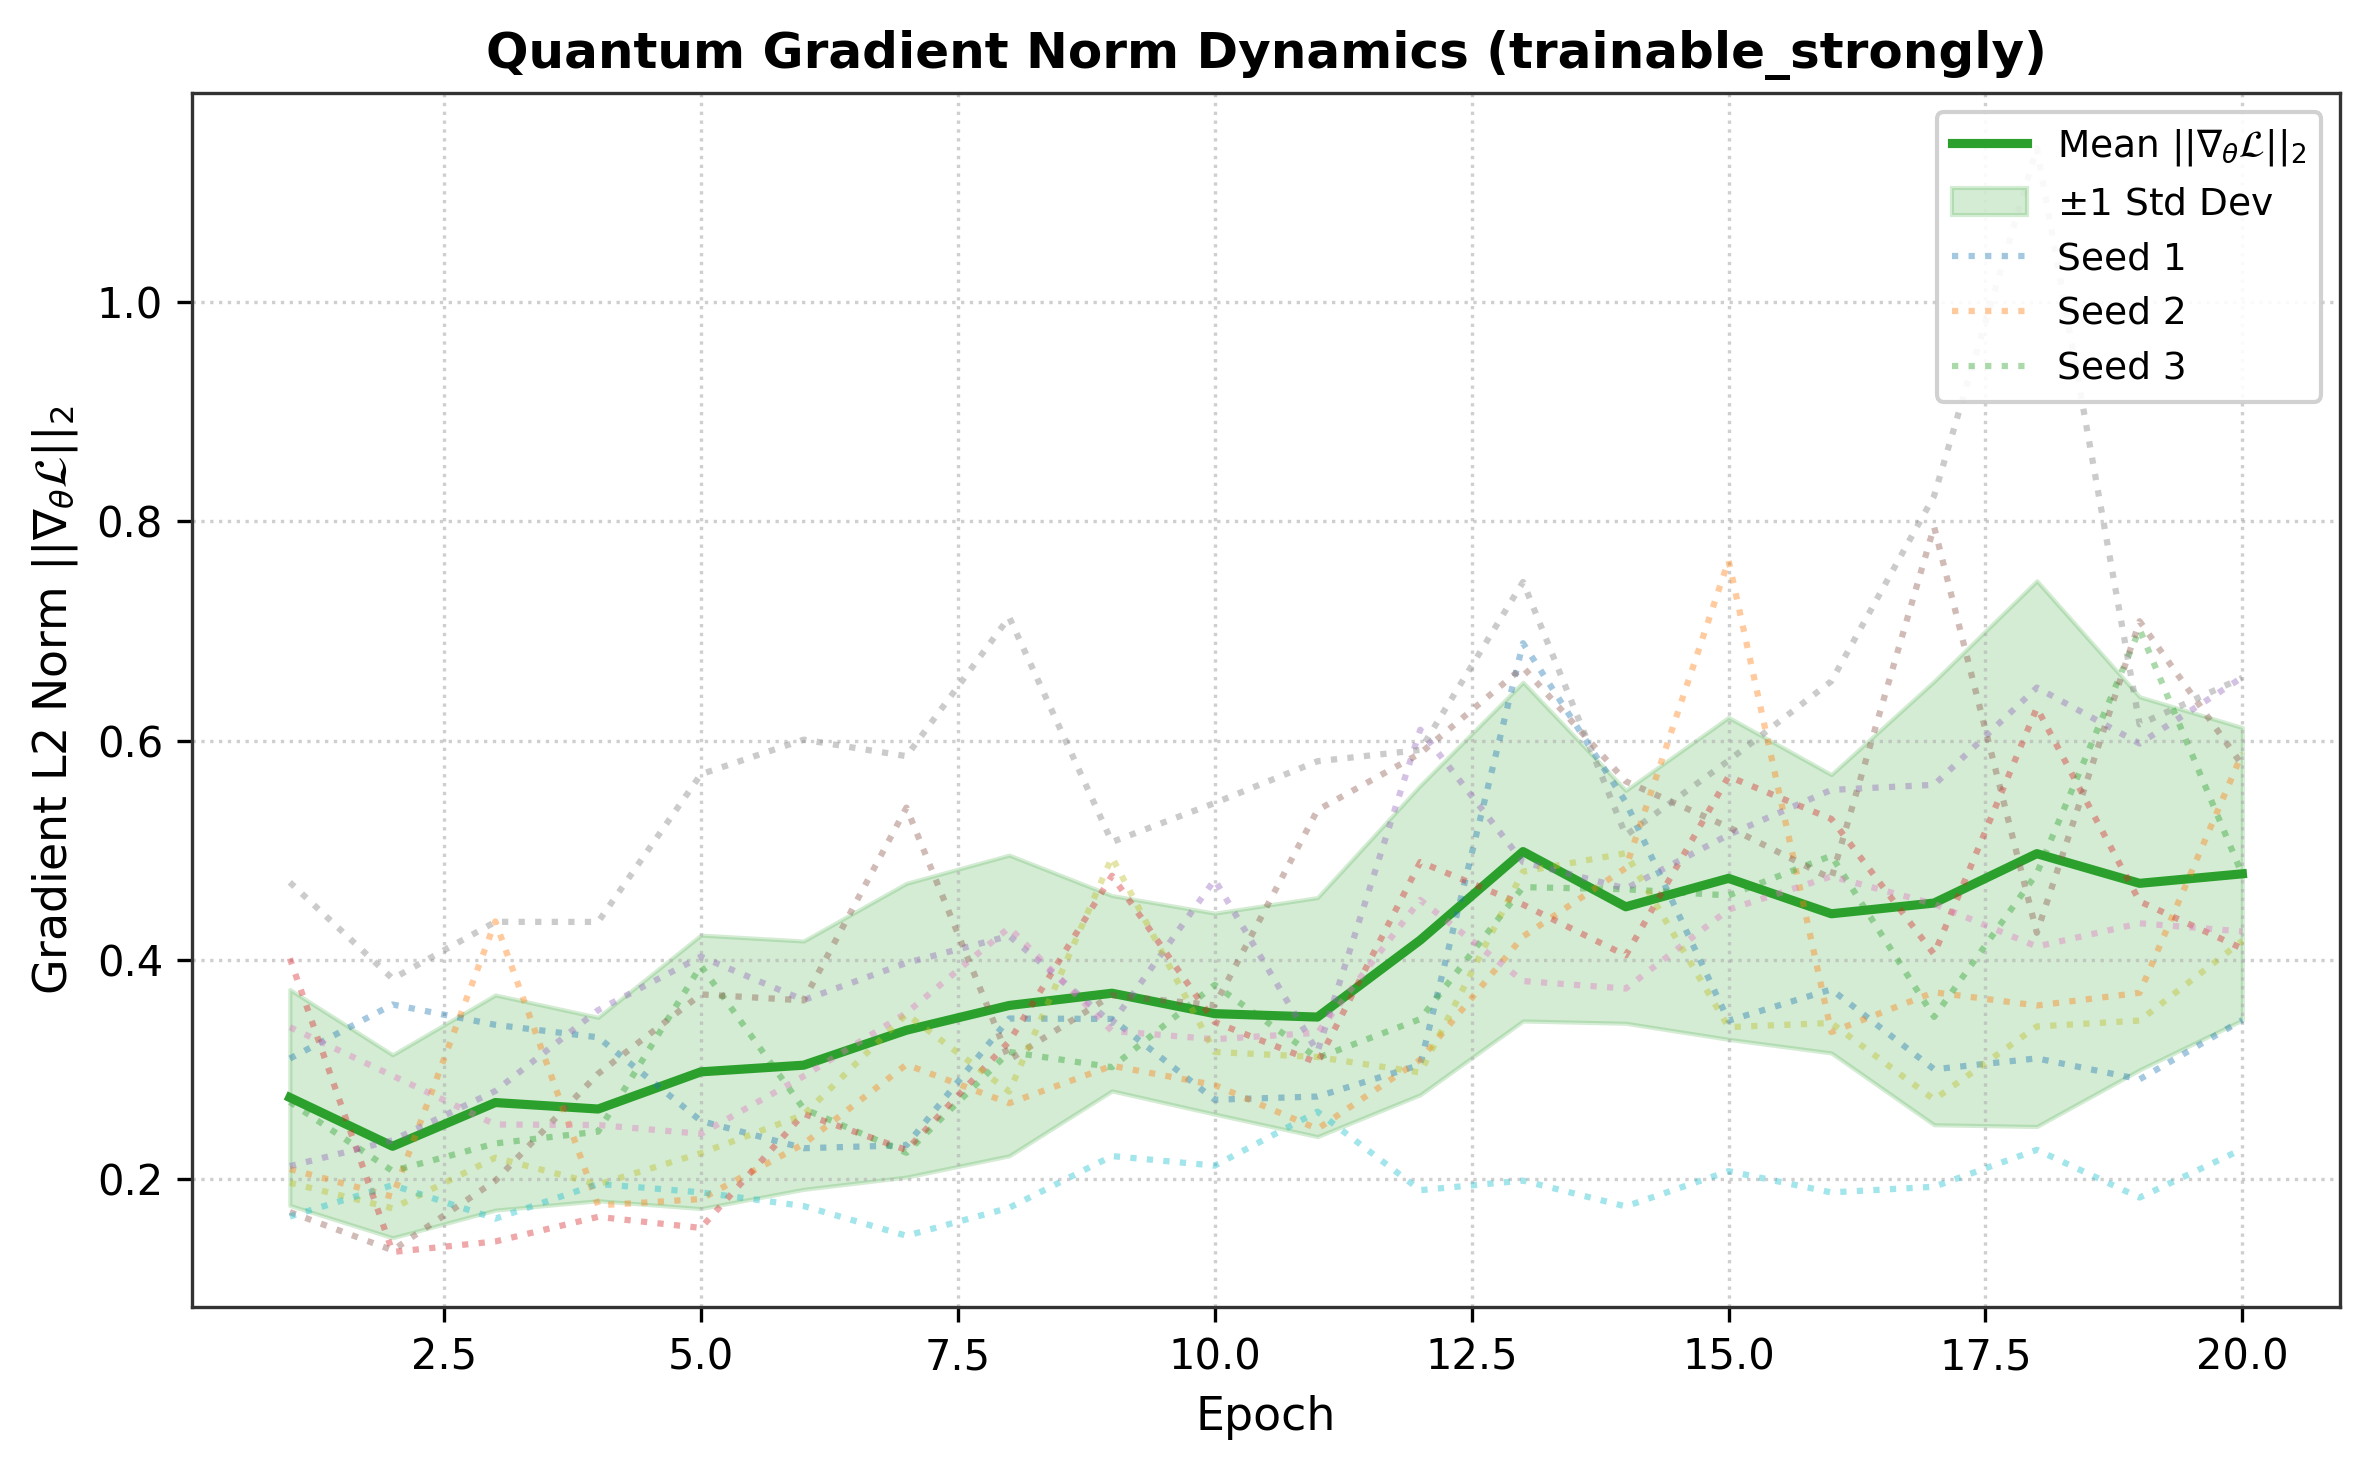
\includegraphics[width=0.48\textwidth]{figures/Fig4d_gradient_norms.png}
\caption{Training and optimization dynamics across 10 seeds: (a) Loss and ROC-AUC convergence on BreastMNIST; (b) Loss and ROC-AUC convergence on OCTMNIST; (c) Quantum rotational angle parameter trajectories $\theta(t)$ over 20 epochs; (d) Parameter gradient $L_2$ norms $\|\nabla_\theta \mathcal{L}\|_2$ confirming healthy gradient flow.}
\label{fig:dynamics}
\end{figure*}

\subsection{Computational Latency \& Hardware Costs}
Table~\ref{tab:latency} breaks down CPU inference latency and training wall-clock time.

\begin{table}[t]
\caption{Inference latency and computational cost on Intel CPU.}
\label{tab:latency}
\centering
\footnotesize
\begin{tabularx}{\columnwidth}{@{}L L C C C@{}}
\toprule
\textbf{Model} & \textbf{Phase} & \textbf{Mean Latency} & \textbf{Ratio} & \textbf{Kernel Params} \\
\midrule
\textbf{Classical CNN} & Forward Pass & \textbf{$0.310\text{ ms}$} & \textbf{$1.0\times$} & $20$ \\
\midrule
\multirow{3}{*}{\textbf{Fixed Quanv}} & FE ($196$ patches) & $220.187\text{ ms}$ & $710.3\times$ & \textbf{$0$} \\
\addlinespace[2pt]
& Classifier Head & $0.034\text{ ms}$ & $0.11\times$ & Identical \\
\addlinespace[2pt]
& \textbf{End-to-End} & \textbf{$220.221\text{ ms}$} & \textbf{$710.4\times$} & \textbf{$0$} \\
\midrule
\textbf{Trainable Quanv} & \textbf{End-to-End} & \textbf{$\sim 220.25\text{ ms}$} & \textbf{$\sim 710.5\times$} & $12 - 24$ \\
\bottomrule
\end{tabularx}
\end{table}

Key computational insights include:
\begin{itemize}
    \item Over $99.98\%$ of execution time is spent on simulating $196$ quantum statevector evolutions on CPU.
    \item Although simulation is $\sim 710\times$ slower than classical convolution, an inference latency of $\approx 0.22\text{ s/image}$ is entirely viable for clinical CAD workflows.
    \item Fixed quanvolutions allow one-time feature precomputation, reducing 10-seed training time to just $18\text{ seconds}$.
\end{itemize}

\section{Discussion}

\subsection{Decoupling Data Regimes: Capacity Bottleneck vs. Regularization}
The divergent outcomes between BreastMNIST and OCTMNIST highlight a fundamental architectural principle:
\begin{itemize}
    \item \textbf{Small Data Regime (BreastMNIST --- 546 train samples, binary):} Classical convolutions with freely unconstrained weights readily overfit spurious artifacts. The fixed 4-qubit quantum transformation acts as a rigid \textbf{Structural Regularizer} in Hilbert space, compressing the optimization search space and resulting in a $\sim 2.73\times$ reduction in variance and peak ROC-AUC ($0.8497$).
    \item \textbf{Large Multi-Class Regime (OCTMNIST --- 3,500 train samples, 4 classes):} Separating 4 subtle retinal pathologies requires high spatial feature flexibility. Shallow 4-qubit kernels hit an \textbf{Expressibility Bottleneck}, whereas classical convolutions scale effectively to dominate the task ($0.7490$ vs. $0.6922$).
\end{itemize}

\subsection{Potency of Quantum Inductive Bias in Zero-Parameter Kernels}
A major finding is that zero-parameter fixed quantum circuits (\texttt{Fixed Basic} and \texttt{Fixed Strongly}) achieved top-tier performance on BreastMNIST, outperforming heavily parameterized trainable counterparts. This confirms that adding trainable parameters to the quantum circuit does not guarantee improved generalization in low-data regimes; an appropriately designed fixed circuit provides sufficient inductive bias with \textbf{strictly zero trainable kernel parameters}.

\subsection{Clinical Relevance in Medical Diagnosis}
In screening scenarios, false negatives are vastly more costly than false positives. Thus, PR-AUC under class imbalance serves as the critical clinical metric. The fact that \texttt{Fixed Strongly Quanvolution} reaches a PR-AUC of $\mathbf{0.9182 \pm 0.0067}$ ($d = +1.332$ over Classical CNN at $0.9057$) demonstrates the unique sensitivity of quantum kernel representations in isolating rare pathological cases.

\section{Threats to Validity \& Limitations}
\begin{enumerate}
    \item \textbf{Resolution \& Patch Size:} This study is limited to $28 \times 28$ MedMNIST images with $2 \times 2$ (4-qubit) patches. Scaling to $224 \times 224$ images will require advanced multi-scale patch partitioning.
    \item \textbf{Simulation Environment:} All experiments were conducted on noiseless statevector simulators (\texttt{default.qubit}). Physical QPU execution will introduce gate errors and readout decoherence.
\end{enumerate}

\section{Conclusion \& Future Work}
This study presented a rigorous, symmetrical benchmark comparing Trainable and Fixed Quanvolutions against a Classical CNN on MedMNIST.

We summarize three primary conclusions:
\begin{enumerate}
    \item \textbf{Quantum advantage is strictly data-regime dependent:} Quanvolution provides significant ranking and stability advantages on small, imbalanced datasets, but classical CNNs decisively dominate on larger multi-class benchmarks.
    \item \textbf{Zero-parameter fixed kernels provide powerful inductive bias:} Fixed circuits deliver superior variance stability ($\sim 2.73\times$ lower std) and top PR-AUC without training kernel parameters.
    \item \textbf{Trainability is localized:} Optimizing quantum rotational angles yields gains only within the same circuit family, failing to outperform optimal fixed baselines.
\end{enumerate}

\textbf{Future Work:} We plan to integrate GPU-accelerated tensor network backends (e.g., NVIDIA cuQuantum) to evaluate noise resilience under realistic NISQ hardware models.

\begin{thebibliography}{00}
\bibitem{litjens2017survey} G.~Litjens et al., ``A survey on deep learning in medical image analysis,'' \textit{Medical Image Analysis}, vol.~42, pp.~60--88, Dec.~2017.
\bibitem{yang2023medmnist} J.~Yang et al., ``MedMNIST v2 - A large-scale lightweight benchmark for 2D and 3D biomedical image classification,'' \textit{Scientific Data}, vol.~10, no.~1, p.~41, Jan.~2023.
\bibitem{esteva2019guide} A.~Esteva et al., ``A guide to deep learning in healthcare,'' \textit{Nature Medicine}, vol.~25, no.~1, pp.~24--29, Jan.~2019.
\bibitem{shorten2019survey} C.~Shorten and T.~M.~Khoshgoftaar, ``A survey on image data augmentation for deep learning,'' \textit{J. Big Data}, vol.~6, no.~1, p.~60, 2019.
\bibitem{biamonte2017quantum} J.~Biamonte et al., ``Quantum machine learning,'' \textit{Nature}, vol.~549, no.~7671, pp.~195--202, Sep.~2017.
\bibitem{cerezo2021variational} M.~Cerezo et al., ``Variational quantum algorithms,'' \textit{Nature Reviews Physics}, vol.~3, no.~9, pp.~625--644, Sep.~2021.
\bibitem{henderson2020quanvolutional} M.~Henderson, S.~Shakya, S.~Pradhan, and T.~Cook, ``Quanvolutional neural networks: powering image recognition with quantum circuits,'' \textit{Quantum Machine Intelligence}, vol.~2, no.~1, p.~2, Jun.~2020.
\bibitem{huang2021power} H.~Y.~Huang et al., ``Power of data in quantum machine learning,'' \textit{Nature Communications}, vol.~12, no.~1, p.~2631, May~2021.
\bibitem{vu2024exploring} T.~H.~Vu, H.~L.~Le, and T.~B.~Pham, ``Exploring the features of quanvolutional neural networks for improved image classification,'' \textit{Quantum Machine Intelligence}, vol.~6, no.~1, p.~15, Feb.~2024.
\bibitem{altares2021automatic} F.~M.~Altares-L{\'o}pez, A.~Ribeiro, and J.~J.~Garc{\'i}a-Ripoll, ``Automatic design of quantum feature maps,'' \textit{Quantum Science and Technology}, vol.~6, no.~4, p.~045015, Jul.~2021.
\bibitem{azevedo2022quantum} F.~S.~Azevedo, A.~Silva, and I.~C.~Oliveira, ``Quantum transfer learning for breast cancer detection,'' \textit{Quantum Information Processing}, vol.~21, no.~3, p.~112, Mar.~2022.
\bibitem{hoang2023efficient} Q.~N.~Hoang, T.~T.~Pham, and D.~N.~M.~Dang, ``Efficient hybrid quantum-classical convolutional neural network with feature propagation layer for multi-class image classification,'' in \textit{Proc. Int. Conf. Adv. Eng. Theory Appl. (AETA)}, 2023.
\bibitem{kubler2021inductive} J.~K{\"u}bler, S.~Buchholz, and B.~Sch{\"o}lkopf, ``The inductive bias of quantum kernels,'' in \textit{Advances in Neural Information Processing Systems (NeurIPS)}, vol.~34, pp.~12661--12673, 2021.
\bibitem{cong2019quantum} I.~Cong, S.~Choi, and M.~D.~Lukin, ``Quantum convolutional neural networks,'' \textit{Nature Physics}, vol.~15, no.~12, pp.~1273--1278, Dec.~2019.
\bibitem{bergholm2018pennylane} V.~Bergholm et al., ``PennyLane: Automatic differentiation of quantum machine learning circuits,'' \textit{arXiv:1811.04968}, 2018.
\bibitem{schuld2019evaluating} M.~Schuld, V.~Bergholm, C.~Gogolin, J.~Izaac, and N.~Killoran, ``Evaluating analytic gradients on quantum hardware,'' \textit{Physical Review A}, vol.~99, no.~3, p.~032331, Mar.~2019.
\bibitem{mcclean2018barren} J.~R.~McClean, S.~Boixo, V.~N.~Smelyanskiy, R.~Babbush, and H.~Neven, ``Barren plateaus in quantum neural network training landscapes,'' \textit{Nature Communications}, vol.~9, no.~1, p.~4812, Nov.~2018.
\end{thebibliography}

\end{document}
